\documentclass{article}
\usepackage[utf8]{inputenc}
\usepackage{amsmath}
\usepackage{tcolorbox}
\usepackage{graphicx}
\usepackage{amsfonts}
\usepackage{amssymb}
\usepackage{tikz}
\usepackage{ebproof}
\usepackage{subfig}

\tcbuselibrary{listings}
\newcommand{\Mod}[1]{\ (\mathrm{mod}\ #1)}
\usetikzlibrary{shapes,positioning,fit,calc}

\begin{document}

\begin{titlepage}
    \begin{center}
        \vspace*{1cm}
            
		\includegraphics[width=0.5\textwidth]{epfl.jpeg}               
            
        \Huge
        \textbf{Advanced Information, Computation and Communication}
            
        \vspace{0.5cm}
        \LARGE
        EPFL - IC
            
        \vspace{0.8cm}
            
        \textbf{Giovanni Ranieri}
            
        \vfill
            
        A summary of AICC main concepts\\
        
		\vspace{0.8cm}     
        
        Course given by professors\\
        Karl Aberer\\
        Bixio Rimoldi\\
        Michael Gastpar
            
        \vspace{0.8cm}
            
    \end{center}
\end{titlepage}

\tableofcontents

\newpage
\section{Propositional Logic}
\subsection{Basic Concepts}
\subsubsection{Proposition}
A proposition is a declarative sentence that is either $ \textbf{true} $ or $ \textbf{false} $. A proposition that cannot be expressed in terms of simpler propositions are called atomic propositions.

\subsubsection{Logical Connectives}
Logical connectives are symbols that are used to connect multiple formulas. The main logical connectives are:
\begin{itemize}
\item The negation $ \neg $
\item The inclusive conjunction $ \wedge $
\item The exclusive conjunction $ \oplus $
\item The disjunction $ \vee $
\item The implication $ \rightarrow $
\item The bi-condition $ \Leftrightarrow $
\end{itemize}
Let $ P $ be the proposition "It rains", then the negation $ \neg P $ is "it not rains".

\subsubsection{Truth Tables}
A truth table is a table that lists all possible values of a compound expression in terms of the different propositions. For example, the truth table of the expression $ P \wedge Q $ is
\renewcommand{\arraystretch}{1.5} % <-- optional a
\begin{center} % <-- optional b
\[ % <-- step a
\begin{array}{|c|c|c|} \hline % <-- steps b, c; optional c, d
P & Q & P \wedge Q\\ \hline
T & T & T\\
T & F & F\\
F & T & F\\
F & F & F\\
\hline
\end{array} % <-- step e
\] % <-- step e
\end{center}
And the main truth tables are:

\renewcommand{\arraystretch}{1.5} % <-- optional a
\begin{center}
\[
\begin{array}{|c|c|c|} \hline % <-- steps b, c; optional c, d
P & Q & P \vee Q\\ \hline
T & T & T\\
T & F & T\\
F & T & T\\
F & F & F\\
\hline
\end{array} \mkern30mu % <-- step e
\begin{array}{|c|c|c|} \hline % <-- steps b, c; optional c, d
P & Q & P \oplus Q\\ \hline
T & T & F\\
T & F & T\\
F & T & T\\
F & F & F\\
\hline
\end{array} \mkern30mu  % <-- step e
\begin{array}{|c|c|c|} \hline % <-- steps b, c; optional c, d
P & Q & P \rightarrow Q\\ \hline
T & T & T\\
T & F & F\\
F & T & T\\
F & F & T\\
\hline
\end{array} \mkern30mu  % <-- step e
\begin{array}{|c|c|c|} \hline % <-- steps b, c; optional c, d
P & Q & P \Leftrightarrow Q\\ \hline
T & T & T\\
T & F & F\\
F & T & F\\
F & F & T\\
\hline
\end{array}  % <-- step e
\]
\end{center}

\subsubsection{Terminology}
\begin{itemize}
\item A \textbf{Tautology} is a proposition always true.
\item A \textbf{Contradiction} is a proposition always false.
\item A \textbf{Contingency} is neither a tautology nor a contradiction.
\end{itemize}

\subsection{Logical Equivalences}
\subsubsection{Definition}
Two propositions are said $ \textbf{equivalent} $ if $ P \Leftrightarrow Q $ is a tautology. We write this like this
\begin{equation}
P \equiv Q
\end{equation}
We can see equivalences in the truth tables too, by checking if the columns in a truth table giving their truth tables agree.

\tcbset{colback=red!5!white,colframe=red!75!black}
\begin{tcolorbox}[width=12.1cm, leftrule=3mm]
$ P \rightarrow Q $ is $ \textbf{NOT} $ equivalent to $ Q \rightarrow P $. But $ P \rightarrow Q \equiv \neg Q \rightarrow \neg P $
\end{tcolorbox}

\subsubsection{Tables of Equivalences}
\begin{figure}[h]
  \hfill\includegraphics[width=0.5\textwidth]{equiv.png}\hspace*{\fill}
  \label{fig:equiv}
\end{figure}  

\subsection{Morgan's Law}
\subsubsection{Definition} 
Let $ P $ and $ Q $ 2 propositions. We can resume the Morgan's Law as
\begin{align}
\neg (P \wedge Q) \Leftrightarrow \neg P \vee \neg Q\\
\neg (P \vee Q) \Leftrightarrow \neg P \wedge \neg Q
\end{align}

\subsubsection{Proof}
\tcbset{colback=gray!5!white,colframe=gray!75!black}
\begin{tcolorbox}[width=12.1cm]
Let $ A = \neg(P \vee Q) $ and $ X \in A $. By definition, $ X \notin (P \vee Q) $. So $ X \notin P $ and $ X \notin Q \Rightarrow X \in \neg P $ and $ X \in \neg Q \Rightarrow X \in \neg P \wedge \neg Q $. We use the same things for the second equivalence.
\end{tcolorbox}

\subsection{Normal Forms}
\subsubsection{Disjunctive Normal Form (DNF)} It's a disjunction of compound expressions where each compound expression is a conjunction of a set of propositional variables of their negation.
\begin{center}
$ (P \wedge \neg Q) \vee (P \wedge R) \vee (Q \wedge T) $
\end{center}

\subsubsection{Conjunctive Normal Form (CNF)} It's a conjunction of compound expressions where each compound expression is a disjunction of a set of propositional variables of their negation.
\begin{center}
$ (P \vee \neg Q) \wedge (P \vee R) \wedge (Q \vee T) $
\end{center}

\begin{tcolorbox}[sharp corners, colback=green!30, colframe=green!80!blue, title=Theorem Of CNF]
Every proposition can be put into a conjunctive normal form.
\end{tcolorbox}

\subsection{Universal and Existential Quantifiers}
\subsubsection{Variables} It's an object that characterize something by properties. For example, in $ Man(x) - \textit{x is a man} $, $ x $ is a variable.

\subsubsection{Predicates} It's a statement that contains a variable and no logical connectives. The example of $ Man(x) $ is a predicate.

\subsubsection{Predicates and Propositional Logic} Let $ M(x) $ and $ N(y) $, 2 predicates. Then $ M(Alice) \wedge N(Bob) $ is a combination of predicates with logical operations.

\subsubsection{Propositional Functions} We can define more general predicates defining functions like $ R(x,y) := P(x) \rightarrow P(y) $.

\subsubsection{Universal Quantifier} The Universal quantifier of a statement is written with the $ \forall $ symbol and it means that $ P(x) $ is true for all values $ x $ from it's domain $ U $.

\subsubsection{Existential Quantifier} The Existential quantifier of a statement is written with the $ \exists $ symbol and it means that $ P(x) $ is true for a value $ x $ from it's domain $ U $.

\subsection{Validity and Satisfiability}
\subsubsection{Statement Valid} A statement involving predicates and quantifiers with all variables bounded is valid if it's true for all domains and every propositional function substituted for the predicates in the assertion.

\subsubsection{Statement Satisfiable} A statement involving predicates and quantifiers with all variables bounded is valid if it's true for some domains. Otherwise it's unsatisfied.

\subsection{The Morgan's Law for Quantifiers}
\renewcommand{\arraystretch}{1.5} % <-- optional a
\begin{center} % <-- optional b
\[ % <-- step a
\begin{array}{|r|c|l|} \hline % <-- steps b, c; optional c, d
Negation & Equivalent Statement\\ \hline
\neg \exists P(x) & \forall x \neg P(x)\\
\neg \forall x P(x) & \exists x \neg P(x)\\
\hline
\end{array} % <-- step e
\] % <-- step e
\end{center}

\tcbset{colback=red!5!white,colframe=red!75!black}
\begin{tcolorbox}[width=12.1cm, leftrule=3mm]
Warning, the ordering of quantifiers is \textbf{critical}.
\end{tcolorbox}

\subsection{Visualization of Quantifiers}

\begin{figure}[!ht]
  \includegraphics[width=\linewidth]{visualization.png}
  \label{fig:visualization}
\end{figure}

\subsection{Proofs}
\subsubsection{Argument} An argument is a sequence of propositions. Every proposition without the final are called premises and the last the conclusion. 
\tcbset{colback=yellow!5!white,colframe=yellow!75!black}
\begin{tcolorbox}[width=12.1cm, leftrule=3mm]
The argument is said valid if and only if the premises imply the conclusion.
\end{tcolorbox}

\subsubsection{Inference Rules} An inference rule is a simple argument form that will be used to construct more complex argument forms. The lines on the fraction bar are propositions and there are put together with AND logic. The proposition under the fraction bar is the implication of the premises over the fraction bar.

\begin{center}
\[
\begin{array}{|c|c|c|c|} \hline
Rules & Name & Rules & Name\\ \hline
\frac{P}{P \vee Q} & Addition & \frac{P \wedge Q}{P} & Simplifation \\
\frac{P \vee Q \textit{ and } \neg P}{Q} & \textit{Disjunctive Syllogism} & \frac{P \rightarrow Q \textit{ and } P}{Q} & \textit{Modus Ponens} \\
\hline
\end{array}
\]
\end{center}

\begin{figure}[h]
  \includegraphics[width=\linewidth]{inferencerule.png}
  \label{fig:visualization}
\end{figure}


\subsubsection{Inference Rules with Quantifiers} An inference rule with quantifiers is an inference rule but we introduced quantifiers in it.

\begin{center}
\[
\begin{array}{|c|c|c|c|} \hline
Rules\\ \hline
\frac{\forall x P(x)}{P(c)} \\
\frac{\exists x P(x)}{P(c) \textit{ for some element c }}\\
\hline
\end{array}
\]
\end{center}


\subsubsection{Type of Proofs}
\begin{itemize}
\item \textbf{Direct proof}: Assume $ P $ is true, then we use rules of inference, axioms till the statement $ Q $ result.
\item \textbf{Proof by Contraposition}: Assume $ \neg Q $ is true, then we use rules of inference, axioms till the statement $ \neg P $ result. Since $ P \rightarrow Q \equiv \neg Q \rightarrow \neg P $
\item \textbf{Proof by Contradiction}: Assume $ P $ and $ \neg Q $ are true, since $ P \rightarrow Q \equiv (P \wedge \neg Q) \rightarrow F  $
\end{itemize}

\newpage
\section{Basic Structures: Sets, Functions, Sequences and Sums}
\subsection{Basics of Sets}
\subsubsection{Definition} A set is an unordered collection of distinct objects (for example numbers).

\tcbset{colback=red!5!white,colframe=red!75!black}
\begin{tcolorbox}[width=12.1cm, leftrule=3mm]
Sets can be elements of sets: $ \{\{a,b,c\},d\} $ and $ \emptyset \neq \{ \emptyset \} $
\end{tcolorbox}

\subsubsection{Set Equality} Let $ A $ and $ B $, 2 sets. $ A $ and $ B $ are equal if and only if $ A $ and $ B $ have the same elements.
\begin{equation}
\forall x(x \in A \longleftrightarrow x \in B)
\end{equation}

\subsubsection{Subset} The set $ A $ is a subset of the set $ B $ if and only if every element of $ A $ is also in $ B $. We write $ A \subseteq B $.
\begin{equation}
\forall x(x \in A \rightarrow x \in B)
\end{equation}

\tcbset{colback=red!5!white,colframe=red!75!black}
\begin{tcolorbox}[width=12.1cm, leftrule=3mm]
Because $ a \in \emptyset $ is always false, the empty set $ \emptyset $ is a subset for all subset $ S $.
\end{tcolorbox}

\subsubsection{Proper Subset} Let $ A $ and $ B $ be 2 sets and let $ A \subseteq B $ but $ A \neq B $, then we say that $ A $ is a proper subset of $ B $, and it's written $ A \subset B $, if and only if
\begin{equation}
\forall x(x \in A \rightarrow x \in B) \wedge \exists x(x \in B \wedge x \notin A)
\end{equation}
  
\subsubsection{Power Set} We define the power set, denoted as $ \mathcal{P}(A) $, as the set of all subsets of a set $ A $. if $ A = \{a,b\} $ then $ \mathcal{P}(A) = \{\emptyset,\{a\},\{b\},\{a,b\}\} $.

\subsubsection{Tuples and Equality of Tuples} The ordered $ n $-tuples $ (a_1,...,a_n) $ is the ordered collection that has $ a_1 $ as it's first element and $ a_n $ for it's last. 2 $ n $-tuples are equal if and only if their corresponding elements are equal.
\\
2-tuples are called \textbf{ordered pairs}.

\subsubsection{Cartesian Product} Let $ A $ and $ B $, 2 sets. We define the Cartesian product of $ A $ and $ B $ as the set of ordered pairs $ (a,b) $ where $ a \in A $ and $ b \in B $, and denoted as $ A \times B $
\begin{equation}
\mathcal{A} \times \mathcal{B} = \{(a,b) | a \in A \wedge b \in B\}
\end{equation}

\tcbset{colback=yellow!5!white,colframe=yellow!75!black}
\begin{tcolorbox}[width=12.1cm, leftrule=3mm]
A subset $ \mathcal{R} $ of the Cartesian product $ \mathcal{A} \times \mathcal{B} $ is called a \textbf{relation} from the set $ \mathcal{A} $ to the set $ \mathcal{B} $.
\end{tcolorbox}
\tcbset{colback=red!5!white,colframe=red!75!black}
\begin{tcolorbox}[width=12.1cm, leftrule=3mm]
Note that in general $ \mathcal{A} \times \mathcal{B} \neq \mathcal{B} \times \mathcal{A} $
\end{tcolorbox}

\subsubsection{Generalization of the Cartesian Product} More generally, we define the Cartesian product of the sets $ A_1,...,A_n $, denoted by $ A_1 \times ... \times A_n $, as the set of ordered $ n $-tuples $ (a_1,...,a_n) $ where $ a_i $ belongs to $ A_i $ for $ i=1,...,n $.
\begin{equation}
A_1 \times ... \times A_n =  \{(a_1,...,a_n) | a_i \in A_i \textit{ for } i=1,...,n\}
\end{equation} 

\subsubsection{Cardinality of Set} The cardinality of a set $ A $, denoted as $ |A| $, is the number of distinct elements in A. We say that the set is finite if there are exactly $ n $ non-negative elements ; otherwise it's infinite.

\tcbset{colback=yellow!5!white,colframe=yellow!75!black}
\begin{tcolorbox}[width=12.1cm, leftrule=3mm]
The cardinality of the Power set $ \mathcal{P}(A) = 2^n $ where $ n $ is the number of elements in $ A $. Also, if $ |A| = n $ and $ |B| = m \Rightarrow |A \times B| = nm $. 
\end{tcolorbox}

\subsection{Set Operations}
\subsubsection{Union} Let $ A $ and $ B $, 2 sets. The union of $ A $ and $ B $, denoted by $ A \cup B $, is the set:
\begin{equation}
\{x | x \in A \vee x \in B\}
\end{equation}  

\subsubsection{Intersection} Let $ A $ and $ B $, 2 sets. The intersection of $ A $ and $ B $, denoted by $ A \cap B $, is the set:
\begin{equation}
\{x | x \in A \wedge x \in B\}
\end{equation}
\\
Sets that have no intersection $ (A \cap B = \emptyset) $ are called \textbf{disjoint}

\subsubsection{Complement} Let $ A $ be a set. The complement of $ A $ with respect to the universe set $ \mathcal{U} $, denoted by $ \bar{A} = \mathcal{U} - A $, is the set:
\begin{equation}
\{x \in \mathcal{U} | x \notin A\}
\end{equation}

\subsubsection{Symmetric Difference} Let $ A $ and $ B $, 2 sets. The symmetric difference of $ A $ and $ B $, denoted by $ A \oplus B $, is the set:
\begin{equation}
(A - B) \vee (B - A)
\end{equation}

\subsubsection{Inclusion-Exclusion Principle} The inclusion-exclusion principle is a principle that represent a counting technique which generalizes the familiar method of obtaining the number of elements in the union of two finite sets. 
\begin{equation}
|A \cup B| = |A| + |B| - |A \cap B|
\end{equation}
\begin{tcolorbox}[sharp corners, colback=green!30, colframe=green!80!blue, title=Cardinality of Sets Union]
Let $ A_1,...,A_n $ be $ n $ finite sets. then $ |A_1 \cup ... \cup A_n| = \sum_{i}^{n}|A_i| - \sum_{1 \leq i < k \leq n}|A_i \cap A_k| + \sum_{i}^{n}|A_i| - \sum_{1 \leq i < j < k \leq n}|A_i \cap A_k \cap A_j| + ... + (-1)^n |\bigcap\limits_{i}^{n}A_i| $ 
\end{tcolorbox}

\subsubsection{Set Identities (Morgan's Law revisited)} Let $ A $ and $ B $, 2 sets. Then
\begin{align}
\overline{A \cap B} = \overline{A} \cup \overline{B}\\
\overline{A \cup B} = \overline{A} \cap \overline{B}
\end{align}
\\
\tcbset{colback=gray!5!white,colframe=gray!75!black}
\begin{tcolorbox}[width=12.1cm]
Let $ \overline{A \cap B} = \{x | x \notin A \cap B\} = \{x | \neg(x \in A \cap B)\} = \{x | \neg(x \in A \wedge x \in B)\} = \{x | \neg x \in A \vee \neg x \in B\} = \{x | x \in \overline{A} \vee x \in \overline{B}\} = \{x | x \in \overline{A} \cup \overline{B}\} = \overline{A} \cup \overline{B} $
\end{tcolorbox}

\subsection{Basics of Functions}
\subsubsection{Definition} A function $ f $ from the set $ A $ to the set $ B $ is an assignment of exactly one element of $ B $ to each element of $ A $.
\begin{align}
f: A \rightarrow B\\
x \longmapsto f(x)
\end{align}
\\
We define $ A $ as the domain $ D(f) $ and $ B $ the image of the co-domain. If $ f(a) = b $, then $ a $ is the pre-image of $ b $ and $ b $ is the image of $ a $ by $ f $.

\subsubsection{Injection of a function} We say that $ f $ is injective, or one-to-one, if and only if
\begin{equation}
f(a) = f(b) \textit{ implies that  } a = b \textit{ and } \forall a,b \in D(f)
\end{equation}

\subsubsection{Surjection of a function} We say that $ f $ is surjective, or onto, if and only if
\begin{equation}
\forall b \in B: \exists a \in A: f(a) = b
\end{equation}

\subsubsection{Bijection of a function} We say that $ f $ is bijective if and only if the function is one-to-one and onto. With this, we can find the \textbf{inversion of the function} $ f^{-1}(x) $
\begin{equation}
f^{-1}(y) = x \Leftrightarrow f(x) = y
\end{equation}

\begin{figure}[h]
\centering
\tikzset{every picture/.style={line width=0.75pt}} %set default line width to 0.75pt        

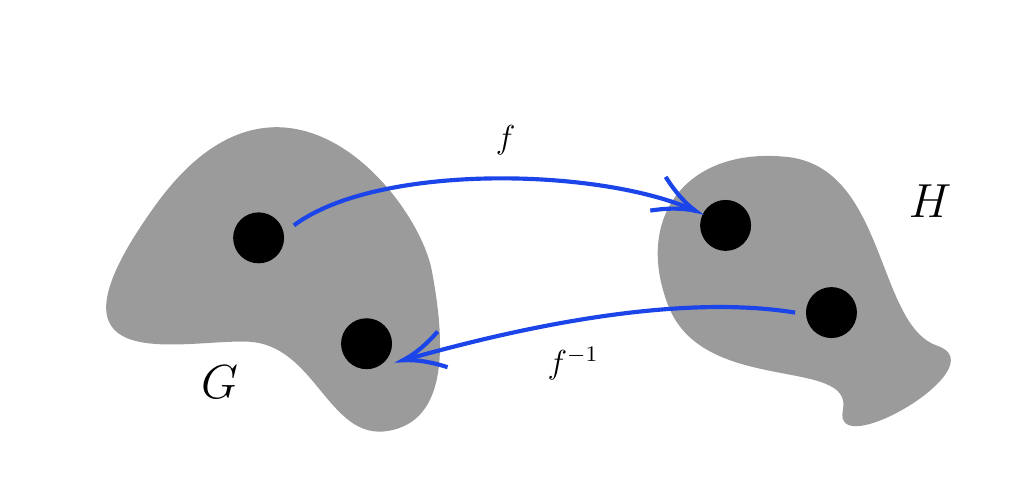
\begin{tikzpicture}[x=0.75pt,y=0.75pt,yscale=-1,xscale=1]

%Shape: Polygon Curved [id:ds23961530607472992] 
\draw  [draw opacity=0][fill={rgb, 255:red, 155; green, 155; blue, 155 }  ,fill opacity=1 ] (96.5,87) .. controls (158,2) and (223,84) .. (229.5,119) .. controls (236,154) and (237.5,191) .. (208.5,196) .. controls (179.5,201) and (173.5,154) .. (140.5,153) .. controls (107.5,152) and (35,172) .. (96.5,87) -- cycle ;
%Shape: Polygon Curved [id:ds5434810466865279] 
\draw  [draw opacity=0][fill={rgb, 255:red, 155; green, 155; blue, 155 }  ,fill opacity=1 ] (343.5,136) .. controls (326.5,93) and (352.5,59) .. (400.5,64) .. controls (448.5,69) and (443.5,145) .. (473,155) .. controls (502.5,165) and (422,212) .. (427.5,186) .. controls (433,160) and (360.5,179) .. (343.5,136) -- cycle ;
%Shape: Circle [id:dp31671262224381147] 
\draw  [fill={rgb, 255:red, 0; green, 0; blue, 0 }  ,fill opacity=1 ] (186,154) .. controls (186,147.37) and (191.37,142) .. (198,142) .. controls (204.63,142) and (210,147.37) .. (210,154) .. controls (210,160.63) and (204.63,166) .. (198,166) .. controls (191.37,166) and (186,160.63) .. (186,154) -- cycle ;
%Shape: Circle [id:dp8563521693066509] 
\draw  [fill={rgb, 255:red, 0; green, 0; blue, 0 }  ,fill opacity=1 ] (410,139) .. controls (410,132.37) and (415.37,127) .. (422,127) .. controls (428.63,127) and (434,132.37) .. (434,139) .. controls (434,145.63) and (428.63,151) .. (422,151) .. controls (415.37,151) and (410,145.63) .. (410,139) -- cycle ;
%Shape: Circle [id:dp23072888295227378] 
\draw  [fill={rgb, 255:red, 0; green, 0; blue, 0 }  ,fill opacity=1 ] (134,103) .. controls (134,96.37) and (139.37,91) .. (146,91) .. controls (152.63,91) and (158,96.37) .. (158,103) .. controls (158,109.63) and (152.63,115) .. (146,115) .. controls (139.37,115) and (134,109.63) .. (134,103) -- cycle ;
%Shape: Circle [id:dp6011767330027358] 
\draw  [fill={rgb, 255:red, 0; green, 0; blue, 0 }  ,fill opacity=1 ] (359,97) .. controls (359,90.37) and (364.37,85) .. (371,85) .. controls (377.63,85) and (383,90.37) .. (383,97) .. controls (383,103.63) and (377.63,109) .. (371,109) .. controls (364.37,109) and (359,103.63) .. (359,97) -- cycle ;
%Curve Lines [id:da8892360866490041] 
\draw [color={rgb, 255:red, 27; green, 68; blue, 233 }  ,draw opacity=1 ][line width=1.5]    (163,97) .. controls (202.4,67.45) and (307.29,68.95) .. (354.39,89.07) ;
\draw [shift={(356.5,90)}, rotate = 204.54] [color={rgb, 255:red, 27; green, 68; blue, 233 }  ,draw opacity=1 ][line width=1.5]    (19.89,-8.92) .. controls (12.65,-4.19) and (6.02,-1.21) .. (0,0) .. controls (6.02,1.21) and (12.65,4.19) .. (19.89,8.92)   ;
%Curve Lines [id:da11406262223883701] 
\draw [color={rgb, 255:red, 27; green, 68; blue, 233 }  ,draw opacity=1 ][line width=1.5]    (404.5,139) .. controls (338.54,128.33) and (250,152.47) .. (218.28,161.23) ;
\draw [shift={(215.5,162)}, rotate = 344.58000000000004] [color={rgb, 255:red, 27; green, 68; blue, 233 }  ,draw opacity=1 ][line width=1.5]    (19.89,-8.92) .. controls (12.65,-4.19) and (6.02,-1.21) .. (0,0) .. controls (6.02,1.21) and (12.65,4.19) .. (19.89,8.92)   ;

% Text Node
\draw (117,163.4) node [anchor=north west][inner sep=0.75pt]  [font=\LARGE]  {$G$};
% Text Node
\draw (458,76.4) node [anchor=north west][inner sep=0.75pt]  [font=\LARGE]  {$H$};
% Text Node
\draw (259,47.4) node [anchor=north west][inner sep=0.75pt]  [font=\large]  {$f$};
% Text Node
\draw (284,154.4) node [anchor=north west][inner sep=0.75pt]  [font=\large]  {$f^{-1}$};


\end{tikzpicture}

\caption{Bijection of a function}
\end{figure}

\subsubsection{Partial Function} A partial function from the set $ A $ to the set $ B $ is an assignment to each element $ a $ in a subset of $ A $, called the domain of definition of $ f $, of a unique element $ b \in B $. For example, the function $ f: \mathbb{Z} \rightarrow \mathbb{R} $ with $ f(x) = \sqrt{x} $ is a partial function because it's only the positive integers that can be send under the sqrt, and the positive integers $ \mathbb{N} $ are a subset of the domain $ \mathbb{Z} $. The definition is fulfilled.

\subsection{Relations}
\subsubsection{Binary Relation} A binary relation $ R $ from a set $ A $ to $ B $ is a subset of the cartesian product of $ A $ and $ B $: $ R \subseteq A \times B $.

\begin{center}
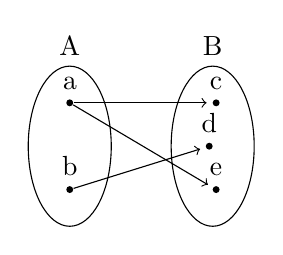
\begin{tikzpicture}
    [
      group/.style={ellipse, draw, minimum height=50pt, minimum width=30pt, label=above:#1},
      my dot/.style={circle, fill, minimum width=2.5pt, label=above:#1, inner sep=0pt}
    ]
    \node (a) [my dot=a] {};
    \node (b) [below=of a, my dot=b] {};
    \node (c) [right=50pt of a, my dot=c] {};
    \node (e) [below=of c, my dot=e] {};
    \node (d) [xshift=-2.5pt, my dot=d] at ($(c)!1/2!(e)$) {};
    \foreach \i/\j in {a/c,a/e,b/d}
      \draw [->, shorten >=2pt] (\i) -- (\j);
    \node [fit=(a) (b), group=A] {};
    \node [fit=(d) (c) (e), group=B] {};
\end{tikzpicture}
\end{center}

\subsubsection{Relations and Functions} A function $ f: A \rightarrow B $ can also be defined as a subset of $ A \times B $, like a relation. A function $ f $ from $ A $ to $ B $ contains one, and only one ordered pair $ (a,b) $ for every element $ a \in A $.
\begin{align}
\forall x[x \in A \rightarrow \exists y[y \in B \wedge (x,y) \in f]]\\
\forall x,y_1,y_2[[(x,y_1) \in f \wedge (x,y_2) \in f] \rightarrow y_1 = y_2]
\end{align}

\tcbset{colback=yellow!5!white,colframe=yellow!75!black}
\begin{tcolorbox}[width=12.1cm, leftrule=3mm]
Relations are more general than functions !
\end{tcolorbox}

\subsubsection{Composition of Relations} Let $ R $ be a relation from the set $ A $ to the set $ B $ and let $ S $ be a relation from the set $ C $ to the set $ D $. The \textbf{composite} of $ R $ and $ S $ is the relation consisting of ordered pairs $ (a,c) $, where $ a \in A $ and $ c \in C $, and for which there exists an element $ b \in B $ such that $ (a,b) \in R $ and $ (b,c) \in S $. We denote the composition of $ R $ and $ S $ like this $ R \circ S $

\begin{figure}[h]
  \includegraphics[width=\linewidth]{relation.png}
  \label{fig:relation}
	
\caption{Example of composition of relations}	
\end{figure}

\subsubsection{Binary Relation on a Set} A binary relation on a set $ A $ is denoted by $ R $ and it's a subset of $ A \times A $.

\subsubsection{Equivalence Relation} Let $ A $ be a set. We say that if a relation is symmetric, transitive and reflexive, then it's an \textbf{equivalence relation}. 2 elements $ a $ and $ b $ that are related by an equivalence are called \textbf{equivalent} and they are written $ a \sim b $.
\begin{itemize}
\item $ R $ is reflexive if and only if $ (a,a) \in R $ $ \forall a \in A $. Reflexive: $ \forall x(x \in A \rightarrow (x,x) \in R) $
\item $ R $ is symmetric if and only if $ (b,a) \in R $ whenever $ (a,b) \in R $. Symmetric: $ \forall x,y((x,y) \in R \rightarrow (y,x) \in R) $
\item $ R $ is transitive if whenever $ (a,b) \in R $ and $ (b,c) \in R $ then $ (a,c) \in R $. Transitive: $ \forall x,y,z((x,y) \in R \wedge (y,z) \in R \rightarrow (x,z) \in R) $
\item $ R $ is anti-symmetric if and only if $ \forall a,b \in A $ if $ (a,b) \in R $ and $ (b,a \in R) $, then $ a = b $. Anti-Symmetric: $\forall x,y((x,y) \in R \wedge (y,x) \in R \rightarrow x = y) $
\end{itemize}

\subsubsection{Number of relation in a set} Let $ A $ be a set. We know that $ A \times A $ has $ |A|^2 $ elements when $ A $ has $ |A| $ elements. This implies

\tcbset{colback=green!5!white,colframe=green!75!black}
\begin{tcolorbox}[sharp corners, colback=green!30, colframe=green!80!blue, title=Number of relation in a set]
The number of relations in a set $ A = 2^{|A|^{2}} $
\end{tcolorbox}

\subsection{Equivalence Classes}
\subsubsection{Definition} Let $ R $ be an equivalence relation on a set $ A $. The set of all elements that are related to an element $ a $ of $ A $ is called an equivalence class of $ a $. The equivalence class of $ a $ with respect to $ R $ is denoted by $ [a]_{R} $. If $ b \in [a]_R $, then $ b $ is called the representative of this equivalence class.

\subsubsection{Example of Equivalence class} Let $ R = \{(a,b) \in \mathbb{R} \times \mathbb{R} | a - b \in \mathbb{Z}\} $. What is the equivalence class of the element 0 ?. $ [0]_R \Rightarrow 0 - b \in \mathbb{Z} \Rightarrow -b \in \mathbb{Z} \Rightarrow b \in \mathbb{Z} $. So in conclusion, we can say that $ [0]_R = \mathbb{Z} $.

\subsection{Equivalence Classes and Partitions}
\subsubsection{Equivalences with Equivalence Classes}
\tcbset{colback=green!5!white,colframe=green!75!black}
\begin{tcolorbox}[sharp corners, colback=green!30, colframe=green!80!blue, title=Equivalences with equivalence classes]
Let $ R $ be an equivalence relation. These statements for elements $ a $ and $ b $ of the set $ A $ are equivalent
\begin{itemize}
\item $ R(a,b) $
\item $ [a] = [b] $
\item $ [a] \cap [b] \neq \emptyset $
\end{itemize}
\end{tcolorbox}

\subsubsection{Partition of a Set} A partition of a set $ S $ is a collection of disjoint non-empty subsets of $ S $ that have $ S $ as their union. Formally for an index set $ I $, the collection of subsets $ A $, where $ i \in I $ forms a partition of $ S $ if and only if
\begin{itemize}
\item $ A_i \neq \emptyset \textit{ } \forall i \in I $
\item $ A_i \cap A_j = \emptyset \textit{ if i = j } $
\item $ \bigcup\limits_{i \in I}A_i = S $
\end{itemize}

\subsubsection{Theorem between Equivalence Classes and Partitions}
\tcbset{colback=green!5!white,colframe=green!75!black}
\begin{tcolorbox}[sharp corners, colback=green!30, colframe=green!80!blue, title=Union of equivalence classes]
Let $ R $ be an equivalence relation. Then the equivalence classes of $ R $ form a partition of $ S $. Conversely, given a partition on $ \{A_i | i \in I\} $ of a set $ S $, there is an equivalence relation on $ R $ that has the sets $ A_i $ as it's equivalence classes.
\end{tcolorbox}

\begin{figure}[h]
  \includegraphics[width=\linewidth]{partitions.png}
  \label{fig:partitions}
	
\caption{Example of partition of a set}	
\end{figure}

\subsubsection{Partial Ordering} A relation $ R $ on a set $ S $ is called a partial ordering if it's reflexive, anti-symmetric and transitive. A set together with a partial ordering $ R $ is called a \textbf{partially ordered set} or \textbf{poset} denoted by $ (S,R) $. Some examples of posets are $ (\mathbb{Z},\geq) $, $ (\mathbb{Z^+}, |) $ or $ (\mathcal{P}(S), \subseteq) $.

\subsubsection{Lattice} A poset in which every pair of elements has both a least upper bound and a greatest lower bound is called a lattice.

\subsubsection{Partial Ordering on Cartesian Product} Given two posets $ (A_1,\prec_1) $ $ (A_2,\prec_2) $, the \textbf{lexicographic ordering on $ A_1 \times A_2 $} is defined by specifying that $ (a_1,a_2) $ is less that $ (b_1,b_2) $ that is $ (a_1,a_2) \prec (b_1,b_2) $, either if $ a_1 \prec_1 b_1 $ or if $ a_1 = b_2 $ and $ a_2 \prec_2 b_2 $.

\begin{figure}[h]
  \includegraphics[width=\linewidth]{lexicographic.png}
  \label{fig:lexicographic}
	
\caption{All ordered pairs less that (3,4)} 	
\end{figure}

\subsubsection{Hasse Diagrams} If a relation is reflexive and transitive, the representation as directed graph can be simplified. If $ R $ is a partial order then we can (a) omit self-loops, (b) omit transitive edges and (c) assume that arrows points upwards.

\begin{figure}%
    \centering
    \subfloat[\centering label 1]{{\includegraphics[width=5cm]{hassediagram1} }}%
    \qquad
    \subfloat[\centering label 2]{{\includegraphics[width=5cm]{hassediagram2} }}%
    \caption{Representation of 2 Hasse Diagrams}%
    \label{fig:hassediagrams}%
\end{figure}

\subsubsection{Comparability} The symbol $ \preceq $ is used to denote the relation in any poset.
\begin{itemize}
\item \textbf{Definition 2:} The elements $ a $ and $ b $ of a poset $ (S, \preceq) $ are \textbf{comparable} if either $ a \preceq b $ or $ b \preceq a $. When $ a $ and $ b $ are elements of $ S $ so that neither $ a \preceq b $ or $ b \preceq a $, then $ a $ and $ b $ are \textbf{incomparable}.
\item \textbf{Definition 3:} If $ (S, \preceq) $ is a poset and every 2 elements of $ S $ are comparable, $ S $ is a \textbf{totally ordered set} and $ \preceq $ is called a \textbf{total order}.
\item \textbf{Definition 4:} $ (S, \preceq) $ is a \textbf{well-ordered set} if it's a poset such that $ \preceq $ is a total ordering and every non-empty subset of $ S $ has a least element.
\end{itemize}

For example, $ (\mathbb{Z}, \leq) $ is totally ordered because with $ a,b \Rightarrow a \leq b,b\leq b $ (or both). $ (\mathbb{Z^+}, |) $ is not totally ordered because for example the element $ (5,7) $, 5 not divide 7 and 7 not divide 5.

\subsection{Sequences}
\subsubsection{Definition} A sequence is a function from a subset of the Integers to a set $ S $. Usually it's either the set $ \mathbb{Z^+} $ or $ \mathbb{N} $. We write $ a_n $ to denote the image $ f(n) $ of $ n $. We can have different progressions:
\begin{itemize}
\item \textbf{Arithmetic Progression:} $ a,a+d,a+2d,... $ gives us the sequence $ f(n) = a + nd $
\item \textbf{Geometrical Progression:} $ a,ar,ar^2,... $ gives us the sequence $ f(n) = ar^n $
\end{itemize}

\subsubsection{Recurrence Relation} A recurrence relation for the sequence $ a_n $ is an expression that express $ a_n $ in terms of a finite number $ k $ of the preceding terms of the sequence. For example 
\begin{equation}
a_n = f(a_{n-1},...,a_{n-k})
\end{equation}

\subsection{Summations}
\subsubsection{Summation Notation} Given a sequence $ a_n $, the notation
\begin{equation}
\sum_{j = m}^{n} a_j
\end{equation}

denotes the sum of the terms $ a_m $, $ a_{m+1} $ ,... ,$ a_n $

\subsubsection{Geometrical Series} if $ a $ and $ r $ are real numbers and $ r \neq 0 $, then
\begin{equation}
\sum_{j=0}^{n} ar^j = \left\{
    \begin{array}{ll}
        \frac{ar^{n+1} - a}{r - 1} & \mbox{if } r \neq 1 \\
        (n + 1)a & \mbox{if } r = 1
    \end{array}
\right.
\end{equation}

Proof:
\tcbset{colback=gray!5!white,colframe=gray!75!black}
\begin{tcolorbox}[width=12.1cm]
Let $ S_n = \sum_{j=0}^{n} ar^j \Leftrightarrow rS_n = r \sum_{j=0}^{n} ar^j = \sum_{j=0}^{n} ar^{j+1} = \sum_{k=1}^{n+1} ar^k = (\sum_{k=0}^{n} ar^k) + (ar^{n+1} -a) = S_n + (ar^{n+1} -a) $. From this equalities, we see that $ rS_n = S_n + (ar^{n+1} -a) $. Solving for $ S_n $ shows that if $ r \neq 1 $, then $ S_n = \frac{ar^{n+1} - a}{r - 1} $. if $ r = 1 $ then $ S_n = \sum_{j=0}^{n} ar^j = \sum_{j=0}^{n} a = (n + 1)a $
\end{tcolorbox}

\subsection{Cardinality with Sets}
\subsubsection{Equal Cardinality}
\begin{tcolorbox}[sharp corners, colback=green!30, colframe=green!80!blue, title=Value of Cardinality between 2 sets]
Let $ A $ and $ B $, 2 sets. Then
\begin{itemize}
\item $ |A| = |B| \Leftrightarrow $ there is a bijection between $ A $ and $ B $
\item If there is an injection from $ A $ to $ B $, then $ |A| \leq |B| $
\end{itemize}
\end{tcolorbox}

\subsubsection{Countable Sets} A set that is either finite of has the same cardinality of $ \mathbb{Z^+} $ is called \textbf{countable}. If it's not, then it's \textbf{uncountable}.
\begin{tcolorbox}[sharp corners, colback=green!30, colframe=green!80!blue, title=Countable Sets]
A set $ S $ is countable if and only if we can list the elements in a sequence indexed, so there exist a bijection $ \mathbb{Z^+} \rightarrow S $
\end{tcolorbox}

\subsubsection{Infinite Countable Sets} When an infinite set is countable, it's cardinality is $ \aleph_0 $, said aleph null. But how it is possible ? The great example of this is the Hilbert Hotel, a hotel with infinite rooms. If the hotel is full and a new guest arrives, we move all guests in the room number $ n + 1 $. With this, we can put the new guest in the first room. In this set, we can count the number of rooms, there is a bijection between the positive integers and the rooms. Even if there is an infinite number of new guests, we can say that the guest in room 1 goes to room 2, the guest in room 2 in the room 4, the 3 into the 6,... and with this, we have an infinite new rooms opened.

\subsubsection{The set of Integers is Countable}
\tcbset{colback=gray!5!white,colframe=gray!75!black}
\begin{tcolorbox}[width=12.1cm]
We define a bijection $ f: \mathbb{Z^+} \rightarrow \mathbb{Z} $ with $ f(n) = \frac{n}{2} $ if $ n $ if even and $ f(n) = \frac{-(n+1)}{2} $ if $ n $ is odd. With this, every element of $ \mathbb{Z} $ is related with an element of $ \mathbb{Z^+} $.
\end{tcolorbox}

\subsubsection{The Set of Rational Numbers is Countable}
\tcbset{colback=gray!5!white,colframe=gray!75!black}
\begin{tcolorbox}[width=12.1cm]
Let us define the mapping $ f: \mathbb{Q} \rightarrow \mathbb{Z} \times \mathbb{N} $ like this:
\begin{equation}
\forall \frac{p}{q} \in \mathbb{Q} : f(\frac{p}{q}) = (p,q)
\end{equation}
where $ \frac{p}{q} $ is in canonical form. Then $ f $ is clearly injective. And from the fact that a cartesian product between 2 countable sets is countable, then we have that $ \mathbb{Z} \times \mathbb{N} $ is countable infinite.
\end{tcolorbox}


\subsubsection{The Set of Real Numbers is Uncountable}
\tcbset{colback=gray!5!white,colframe=gray!75!black}
\begin{tcolorbox}[width=12.1cm]
The proof is based on the Cantor Diagnalization. We will prove that the interval $ [0,1[ \in \mathbb{R} $ is uncountable. Let us write some numbers from this interval.
\begin{center}
$ r_1 = 0.046436 $
$ r_2 = 0.354367 $
$ r_3 = 0.014054 $
$ r_4 = 0.463256 $
$ r_5 = 0.963621 $
$ ... $
$ r_n = 0.r_{n1}r_{n2}... $
\end{center}
Now let us create the number $ x \in [0,1[ $ formed with the $ k $-position of the numbers written above. Here we take the first 1 number after the dot of the $ r_1 $, so 0. Then we take the second number after the dot of $ r_2 $, and so on. And now we say that if the number is 4, we keep 4 and otherwise, we put a 3. We create here the number $ x = 0.3433 \in [0,1[ $. But here $ x $ is clearly not in the sequence formed above. he cannot be $ r_1 $ because the first number after the dot is different, same for the second, the third number,... We prove that we create a new number and so we cannot create a bijection from the positive integers !
\end{tcolorbox}


\newtcblisting{mylisting}{
  listing only,
  hbox,
  colframe=cyan,
  colback=cyan!10,
  listing options={
    basicstyle=\small\ttfamily,
    breaklines=true,
    columns=fullflexible
  },
}

\newpage
\section{Algorithms}
\subsection{Introduction and Examples}
\subsubsection{Definition} An algorithm is a finite set of well-defined, computer-implementable instructions to perform a specified task. Algorithms can be expressed in pseudo-code.
\begin{mylisting}
	procedure max(a_1,...,a_n : integers)
		tmp_max := a_1
		for(i := 2 to n)
			if(tmp_max < a_i) then tmp_max := a_i
			
		return tmp_max
\end{mylisting}

\subsubsection{Binary Search} It's a simple algorithm of search for an element in a list of numbers in increasing order that works with the fact that at each step, we divide the set of research in 2 until we find what we want. With numbers in increasing order, let us define that we want the number 12 in the interval $ [1,20] $. First step, we take the middle of the interval, so 10. 12 is greater than 10, so we search in the subset $ [10,20] $. Now we take the middle of this interval, so 15. 12 is less that 15 so know we take the subset $ [10,13] $. And so on until we find the good number.

\subsubsection{Insertion Sort} It's a good algorithm for sorting a list of numbers. The algorithm begins with the second element and compare it with the first element. If the second is lower that the first, it inverses the 2 elements, otherwise it does nothing. Next, the third element is compared with the 2 first elements and put where it has to be and so on.

\begin{mylisting}
	procedure insertion_sort(a_1,...,a_n : real numbers with n >= 2)
		for(j := 2 to n)
			i := 1
			while(a_j > a_i and i < j)
				i := i + 1
			m := a_j
			for(k := 0 to j - i - 1)
				a_{j-k} := a_{j-k-1}
			a_i := m				
\end{mylisting}

\subsubsection{Greedy Algorithm} A greedy algorithm will take the "best choice" at each step but it won't always produce an optimal solution.

\subsection{Matching}
\subsubsection{Definition} Given a finite set $ A $, a matching of $ A $ is a set of (unordered) pairs of distinct elements of $ A $ where any element occurs in at most one pair. For example, $ (\{(1,2),(3,4)\}) $ is a matching but not $ (\{(2,2),(2,4)\}) $.

\subsubsection{Maximum Matching} A maximum matching is a matching that contains the largest possible number of pair. For example $ (\{(1,2),(3,4)\}) $ with the elements $ \{1,2,3,4\} $.


\subsubsection{Stable Matching} Task: Pair elements from equally sized two groups considering their preferences for members of the other group so that there are no ways to improve the preferences. This notion is not really hard to understand. A stable matching is the fact that pairs of elements from 2 sets with the same cardinality are stable, so no element from a pair wants to be more with an other element of an other pair than the element with him. If we have the pairs $ (a,b) $ and $ (c,d) $, and $ a $ likes more $ c $ than $ b $, and $ c $ likes more $ a $ than $ d $, we have an unstable matching...

\subsubsection{Preference List} A preference list $ L_x $ defines for every element $ x \in A $ the order $ m $ in which the element prefers to be paired with. $ x \in A $ prefers $ y $ to $ z $ if $ y $ precedes $ z $ on $ L_x $.

\subsubsection{Marriage Problem} Given a set with even cardinality, partition $ A $ into two disjoint subsets $ A_1 $ and $ A_2 $ with $ A_1 \cup A_2 = A $ and $ |A_1| = |A_2| $. A \textbf{matching} is a bijection from the elements of one set to the elements of the other set. That means that pairs can only consist of one element of $ A_1 $ and $ A_2 $ each.

\subsubsection{Gale-Shapley Algorithm (proof of existence of stable maximum matching)} Let $ M $ be the set of pairs under construction. Initially, $ M = \emptyset $
\begin{mylisting}
	while M < |A_1|:
		Select an unpaired x in A_1
		Let x propose to the first element y in A_2 on L_x:
		
		if(y is unpaired)
			Add (x,y) to M
		else
			Let z in A_1 be the element that y is paired with to (ie. (y,z) in M)
			if(z precedes x on L_x)
				Remove y from L_x
			else
				Replace	(y,z) in M by (x,y) and remove y from L_x				
\end{mylisting}

\begin{figure}[ht]
  \includegraphics[width=\linewidth]{galeshapley.png}
  \label{fig:galeshapley}
	
\caption{Gale-Shapley Algorithm} 	
\end{figure}

\subsection{Growth Of Functions}
\subsubsection{Introduction} In computer science, we want to describe the way that a function grows. We want to characterize the efficiency of algorithms by this growth of functions.

\subsubsection{Big-O Notation} The big-O notation is used to describe the limiting behaviour of a function when the arguments tend towards a particular value or infinity. It describes the upper limit. We say that $ f(x) $ is $ \mathcal{O}(g(x)) $ if there are constants $ C $ and $ k $ such that
\begin{equation}
|f(x)| \leq C|g(x)| \textit{  } \forall x > k
\end{equation}
$ C $ and $ k $ are called \textbf{witnesses}.

\subsubsection{Examples of big-O} $ f(x) = x^2 + 2x + 1 $ is $ \mathcal{O}(x^2) $
\tcbset{colback=gray!5!white,colframe=gray!75!black}
\begin{tcolorbox}[width=12.1cm]
If $ x > 1 $ then $ x < x^2 $ and $ 1 < x^2 $. Therefore
\begin{equation}
0 \leq f(x) = x^2 + 2x + 1 \leq x^2 + 2x^2 + x^2 = 4x^2
\end{equation}
We choose $ C = 4 $ and $ k = 1 $.
\end{tcolorbox}

\begin{figure}[h]
  \includegraphics[width=\linewidth]{bigo.png}
  \label{fig:bigo}
	
\caption{Graph of the complexity of the function $ f(x) $} 	
\end{figure}

\subsubsection{Big-O Estimation for Polynomials}
\begin{tcolorbox}[sharp corners, colback=green!30, colframe=green!80!blue, title=Complexity of Polynomials]
Let $ p(x) = a_{n}x^{n} + a_{n-1}x^{n-1} + ... + a_{1}x + a_0 $ be a polynomial with $ a_i \in \mathbb{R} $ and $ a_n \neq 0 $. Then $ p(x) $ is $ \mathcal{O}(x^n) $
\end{tcolorbox}

\subsubsection{Big-O Examples}
\begin{itemize}
\item $ \forall u > v \in \mathbb{R} $, $ n^v $ is $ \mathcal{O}(n^u) $ but $ n^u $ is not $ \mathcal{O}(n^v) $
\item $ \forall a > 0, b > 0, u > v \in \mathbb{R} $, $ \log_b(n^v) $ is $ \mathcal{O}(\log_b(n^u)) $ and $ \log_b(n^u) $ is $ \mathcal{O}(\log_b(n^v)) $
\item $ n! $ is $ \mathcal{O}(n^n) $
\item $ \log(n!) $ is $ \mathcal{O}(\log(n)) $
\end{itemize}

\subsubsection{Combination of Functions}
\begin{itemize}
\item if $ f(x) $ is $ \mathcal{O}(g(x)) $ and $ g(x) $ is $ \mathcal{O}(h(x)) \Rightarrow f(x) $ is $ \mathcal{O}(h(x)) $
\item If $ f_1(x) $ is $ \mathcal{O}(g_1(x)) $ and $ f_2(x) $ is $ \mathcal{O}(g_2(x)) \Rightarrow (f_1(x)f_2(x)) $ is $ \mathcal{O}(g_1(x)g_2(x)) $
\item If $ f_1(x) $ and $ f_2(x) $ are $ \mathcal{O}(g(x)) \Rightarrow (f_1(x) + f_2(x)) $ is $ \mathcal{O}(g(x)) $
\item If $ f_1(x) $ is $ \mathcal{O}(g_1(x)) $ and $ f_2(x) $ is $ \mathcal{O}(g_2(x)) \Rightarrow (f_1(x) + f_2(x)) $ is $ \mathcal{O}(max(g_1(x),g_2(x))) $
\end{itemize}

\subsubsection{Big-Omega Notation} The big-$ \Omega $ notation is used to describe the limiting behaviour of a function when the arguments tend towards a particular value or infinity. It not describe the upper limit but the lower limit. We say that $ f(x) $ is $ \Omega(g(x)) $ if there are constants $ C $ and $ k $ such that
\begin{equation}
|f(x)| \geq C|g(x)| \textit{  } \forall x > k
\end{equation}
$ C $ and $ k $ are called \textbf{witnesses}

\begin{tcolorbox}[sharp corners, colback=green!30, colframe=green!80!blue, title=Equivalence Big-O and Big-Omega]
$ f(x) $ is $ \Omega(g(x)) \Leftrightarrow g(x) $ is $ \mathcal{O}(f(x)) $
\end{tcolorbox}

\subsubsection{Example of Big-Omega} The function $ f(x) = x^3 + 8x^2 + 7 $ is $ \Omega(x^3) $ because $ g(x) = x^3 $ is $ \mathcal{O}(x^3 + 8x^2 + 7) $

\subsubsection{Big-Theta Notation} The big-$ \Theta $ notation is used to describe a function that is $ \mathcal{O} $ something and $ \Omega $ something. By definition we describe the Theta notation by this
\begin{equation}
C_1|g(x)| \leq |f(x)| \leq C_2|g(x)| \textit{ if } x > k
\end{equation}
$ C $ and $ k $ are called \textbf{witnesses}. In particular
\begin{tcolorbox}[sharp corners, colback=green!30, colframe=green!80!blue, title=Big-Theta Definition]
$ f(x) $ is $ \Theta(g(x)) $ if $ f(x) $ is $ \mathcal{O}(g(x)) $ and $ f(x) $ is $ \Omega(g(x)) $
\end{tcolorbox}

\begin{tcolorbox}[sharp corners, colback=green!30, colframe=green!80!blue, title=Implication of Theta Notation]
When $ f(x) $ is $ \Theta(g(x)) $, then $ g(x) $ is $ \Theta(f(x)) $. 
\end{tcolorbox}

\begin{tcolorbox}[sharp corners, colback=green!30, colframe=green!80!blue, title=Equivalence of Theta Notation]
$ f(x) $ is $ \Theta(g(x)) \Leftrightarrow f(x) $ is $ \mathcal{O}(g(x)) $ and $ g(x) $ is $ \mathcal{O}(f(x)) $
\end{tcolorbox}

\subsubsection{Big-Theta Estimation for Polynomials}
\begin{tcolorbox}[sharp corners, colback=green!30, colframe=green!80!blue, title=Complexity of Polynomials]
Let $ p(x) = a_{n}x^{n} + a_{n-1}x^{n-1} + ... + a_{1}x + a_0 $ be a polynomial with $ a_i \in \mathbb{R} $ and $ a_n \neq 0 $. Then $ p(x) $ is $ \Theta(x^n) $
\end{tcolorbox}

\subsubsection{Little-o Notation} The little-o notation describes the growth of functions too but in a different way. We say that $ f(x) $ is $ o(g(x)) $ if $ g(x) $ growth faster as $ f(x) $. In particular, $ f(x) $ is $ o(g(x)) $ if
\begin{equation}
\lim_{x \rightarrow \infty}\frac{f(x)}{g(x)} = 0
\end{equation}

\subsection{Complexity of Algorithms}
\subsubsection{Definition} In computer science, we want to know the behaviour of an algorithm for large values when we want to solve a problem. We want to describe the algorithm in terms of the time to solve a problem depending of the input size. The case that we are interested is when the input size is very big and we want to know if algorithms with this size of inputs are efficient. In computer science, we talk about \textbf{computational complexity}. This computational complexity can be separated in 2 parts: \textbf{time complexity}, how much an algorithm take time to solve a problem, and \textbf{space complexity}, the resources that the algorithm must have to solve a problem. We will focus on the first one.

\subsubsection{Time Complexity} The time complexity corresponds to the number of operations performed, and we will use the big-O and big-$ \Theta $ notations to describe it. For this, we assume that all operations take the same time (addition, multiplication, ...). In the problem of complexity, we will focus on the \textbf{Worst-case time} that is, for a given problem with an algorithm to solve it, we will take the upper bound on the number of operations.

\subsubsection{Example of Worst-case complexity (1)} if we take the pseudo-code for the max of a list of numbers:
\begin{mylisting}
	procedure max(a_1,...,a_n : integers)
		tmp_max := a_1
		for(i := 2 to n)
			if(tmp_max < a_i) then tmp_max := a_i
			
		return tmp_max
\end{mylisting}
We see that the $ max < a_i $ is made $ n - 1 $ times. Each time $ i $ is incremented, we have a comparison to see if $ i \leq n $, so $ n - 1 $. One last comparison is made to see if $ i > n $. So in total, we have $ 2(n - 1) + 1 = 2n - 1 $ made. We can conclude that the complexity of this algorithm is $ \Theta(n) $.

\subsubsection{Example of Worst-case complexity (2)} if we take the pseudo-code for the insertion sort algorithm:
\begin{mylisting}
	procedure insertion_sort(a_1,...,a_n : real numbers with n >= 2)
		for(j := 2 to n)
			i := 1
			while(a_j > a_i and i < j)
				i := i + 1
			m := a_j
			for(k := 0 to j - i - 1)
				a_{j-k} := a_{j-k-1}
			a_i := m				
\end{mylisting}
We see first that we have $ n - 1 $ passes for the first loop from $ j = 2 $ to $ n $. In each pass, the while and the for loop inside are executed at most $ j $ times. Since $ 2(2+3+...+n) = n(n + 1) - 2 $, the complexity is $ \Theta(n^2) $.

\subsubsection{Summary of Complexity for some Algorithms}
\renewcommand{\arraystretch}{1.5} % <-- optional a
\begin{center} % <-- optional b
\[ % <-- step a
\begin{array}{|c|c|c|c|} \hline % <-- steps b, c; optional c, d
\textit{Algorithm} & \textit{Time Complexity} & Algorithm & \textit{Time Complexity}\\ \hline
\textit{Linear Search} & \Theta(n) & \textit{Binary Search} & \Theta(log(n))\\
\textit{Bubble Sort} & \Theta(n^2) & \textit{Insertion Sort} & \Theta(n^2)\\
\hline
\end{array} % <-- step e
\] % <-- step e
\end{center}

\subsubsection{Hierarchy of Functions} Non-exhaustive list of complexity of functions
\begin{enumerate}
\item Constant: $ \mathcal{O}(1) $
\item Logarithm: $ \mathcal{O}(\log(x)) $
\item Poly-logarithm: $ \mathcal{O}(\log(x)^n) $
\item Linear: $ \mathcal{O}(x) $
\item Linear-arithmetic: $ \mathcal{O}(x\log(x)) $
\item Polynomial: $ \mathcal{O}(x^n) $
\item Exponential: $ \mathcal{O}(n^x) $
\end{enumerate}

\newpage
\section{Induction and Recursion}
\subsection{Mathematical Induction}
\subsubsection{Definition} The principle of mathematical induction is that we want to prove that something is true for a value $ k + 1 $ assuming a certain base and that the proposition $ P(n) $ is true for $ P(k) $. So we have a \textbf{basic step} (test the proposition for a small value), the \textbf{inductive hypothesis} (we assume that the proposition is true for a $ k $) and the \textbf{inductive step} (prove that the proposition is true for the value $ k + 1 $).

\subsubsection{Induction as Inference Rule} The mathematical induction can be described as the rule of inference
\begin{equation}
(P(1) \wedge \forall k(P(k) \rightarrow P(k + 1))) \rightarrow \forall n \textit{ } P(n)
\end{equation}

\subsubsection{Why Induction is Valid ?} The mathematical induction is valid by the well-ordering property (an axiom for the set of positive integers) that says: every non-empty subset of $ \mathbb{N} $ contains a least element. Mathematical induction is equivalent to this.

\subsubsection{Example of Induction} We want to prove this following sum
\begin{center}
$ P(n): \sum_{i=1}^n i = \frac{n(n + 1)}{2} $
\end{center}
First the basic step: $ P(1) = \sum_{i=1}^{1} i = 1 = \frac{1(2)}{2} $ so it's good. Let assume that the formula is true for $ P(k) $ so that $ \sum_{i=1}^k i = \frac{k(k+1)}{2} $. Let's start the inductive step: 
\begin{center}
$ \sum_{i=1}^{k+1} i = \sum_{i=1}^{k}i + (k + 1) = \frac{k(k + 1)}{2} + (k + 1) = \frac{k(k + 1) + 2(k + 1)}{2} = \frac{(k + 1)(k + 2)}{2} = P(k + 1) $
\end{center}

\subsubsection{Example of Induction with Sets} The theorem is that for a finite set $ S $, the number of subset of $ S $ is $ 2^n $ where $ n $ is it's cardinality. The basic step is for example $ P(0) $ and it's true because the empty set $ \emptyset $ does not have elements and so the unique subset is itself so $ 2^0 = 1 $. Now let's note the inductive hypothesis, so that every set has $ 2^k $ subsets with $ k $ as cardinality. Now let's move on the inductive step. Let $ T $ be a set with $ k + 1 $ elements. Let $ S $ be the set as $ T = S \cup {a} $ for an element $ a \in T $ and so $ S = T - {a} $. Hence, $ |S| = k $ (because $ |T| = k + 1 $). Now for each subset $ X $ of $ S $, we can have two subset of $ T $: $ X $ and $ X \cup {a} $. By inductive step, $ S $ has $ 2^k $ subsets. And so since $ T $ has 2 subsets for each subsets of $ S $, the number of subsets of $ T $ is $ 2*2^k = 2^{k+1} $.

\subsubsection{Strong Induction} To prove that a proposition $ P(n) $ is true for all $ n $, we say that
\begin{equation}
\forall k \textit{ }([P(1) \wedge ... \wedge P(k)] \rightarrow P(k + 1)) 
\end{equation}
We say that the strong induction is the complete mathematical induction.

\subsection{Recursive Definitions and Structural Induction}
\subsubsection{Recursive Defined Function} A recursive of a function $ f $, with non-negative integers as domain, consists of 2 steps
\begin{enumerate}
\item Basic step: specify the value of the function at zero.
\item Recursive step: Give a rule for finding the next value from it's last values. For example, the function $ f(0) = 3 $ and $ f(n + 1) = 2f(n) + 1 $.
\end{enumerate}
We can write the basic recursive defined function for sums
\begin{equation}
\sum_{k=0}^{n+1} a_k = (\sum_{k=0}^n a_k) + a_{n+1}
\end{equation}

\subsubsection{Recursively Defined Sets and Structures} Same as the recursive defined functions, we can say that there is 2 steps:
\begin{enumerate}
\item Basic step specifies an initial collection of elements
\item Recursive step gives the rules for forming new elements in the set from those already in the set.
\end{enumerate}
The basic example is the formation of the set $ \mathbb{N} $.
\begin{itemize}
\item Basic step: $ 0 \in \mathbb{N} $
\item Recursive step: If $ n \in \mathbb{N} $ then $ n + 1 \in \mathbb{N} $.
\end{itemize}

\subsection{Recursive Algorithms}
\subsubsection{Definition} An algorithm is called \textbf{recursive} if it solves a problem by reducing it to an instance of the same problem with smaller input. The basic example of this is the factorial algorithm
\begin{mylisting}
	factorial(n):=
		if(n = 0)
			then return 1
		else
			then return n * factorial(n - 1)				
\end{mylisting}

\subsubsection{Recursive Algorithms Better Than Others} Let's write a recursively algorithm for computing powers of a number.
\begin{mylisting}
	power(a,n):=
		if(n <= 1)
			then return 1
		else
			then return a * power(a,n-1)				
\end{mylisting}
But this algorithm is not really good. Let's write a better algorithm:
\begin{mylisting}
	nice_power(a,n):=
		if(n <= 1)
			then return 1
		else
			then return (a power n&1) *
			nice_power(a, floor of n/2) square				
\end{mylisting}

\begin{figure}%
    \centering
    \subfloat[\centering Simple Algorithm]{{\includegraphics[width=5cm]{power} }}%
    \qquad
    \subfloat[\centering Better Algorithm]{{\includegraphics[width=5cm]{nice_power} }}%
    \caption{Comparison between 2 recursive algorithms for computing powers of a number}%
    \label{fig:powers}%
\end{figure}

\subsubsection{Difference between Recursion and Induction} Recursion and Induction are not the same things when we talk about resolving a problem. The first reduces a problem of any size to the smallest one possible. The second extends this ability to problems of any size. In consequence, a recursively defined function can be described in two ways: recursively of iteratively.

\begin{mylisting}
	iterative_fibonacci(n):=
		if(n=0) then return 1
		else
			previous := 0
			current := 1
			for(i=0 to n-1)
				next := previous + current
				previous := current
				current := next
			return current				
\end{mylisting}
\begin{mylisting}
	recursive_fibonnaci(n):=
		if(n <= 1) then return 1
		else return recursive_fibonnaci(n-1) +
		 recursive_fibonnaci(n-2)			
\end{mylisting}

\section{Number Theory and Group Theory}
\subsection{Division}
\subsubsection{Division} Let $ a,b \in \mathbb{Z} $ and $ a \neq 0 $. We say that a number $ a $ divides $ b $ if there is an integer c such that $ b = ac $. We use the notation $ a | b $ to say that $ a $ divides $ b $.

\subsubsection{Properties of Division} We can list some properties of division
\begin{itemize}
\item $ a | c $ and $ a | b $ then $ a | (b+c) $
\item $ a | c $ then $ a | bc $, $ \forall b \in \mathbb{Z} $
\item $ a | c $ and $ c | b $ then $ a | b $ (transitivity)
\end{itemize}
Proof for the first:

\tcbset{colback=gray!5!white,colframe=gray!75!black}
\begin{tcolorbox}[width=12.1cm]
Suppose that $ a|b $ and $ a|c $. So there exists integers $ s $ and $ t $ such that $ b = as $ and $ c = at $. Hence $ b + c = as + at = a(s+t) $. Hence $ a|(b+c) $
\end{tcolorbox}

\tcbset{colback=yellow!5!white,colframe=yellow!75!black}
\begin{tcolorbox}[width=12.1cm, leftrule=3mm]
Let $ a,b \in \mathbb{N_+} $. if $ a|c $ and $ b|c $, it \textbf{not} implies that $ ab|c $. To have that we must have $ gcd(a,b) = 1 $.
\end{tcolorbox}

\subsubsection{Division Algorithm}
\begin{tcolorbox}[sharp corners, colback=green!30, colframe=green!80!blue, title=Division Algorithm]
If $ a $ is an integer and $ d $ a positive integer, then there are unique integers $ q $ and $ r $ with $ 0 \leq r < d $ such that $ a = dq + r $
\end{tcolorbox}

\subsection{Modular Arithmetic}
\subsubsection{Congruence Relation} If $ a,b \in \mathbb{Z} $ and $ m > 0 $, then we say that $ a $ is congruent to $ b $ modulo $ m $ if $ m|a-b $ and we write $ a \equiv b \Mod m $. For example, $ 17 \equiv 5 \Mod 6 $ because $ 6 | 17-5 $.

\begin{tcolorbox}[sharp corners, colback=green!30, colframe=green!80!blue, title=Congruence Equivalence]
$ a \equiv b \Mod m \Leftrightarrow a \Mod m = b \Mod m $
\end{tcolorbox}

\subsubsection{Congruences of Sums and Products}
\begin{tcolorbox}[sharp corners, colback=green!30, colframe=green!80!blue, title=Congruence of Sums and Products]
Let $ m > 0 $ with $ a \equiv b \Mod m $ and $ c \equiv d \Mod m $ then
\begin{itemize}
\item $ a + c \equiv (b + d) \Mod m $
\item $ ac \equiv (bd) \Mod m $
\end{itemize}
\end{tcolorbox}

\tcbset{colback=red!5!white,colframe=red!75!black}
\begin{tcolorbox}[width=12.1cm, leftrule=3mm]
Dividing a congruence by an integer will not always produce a valid congruence!
\end{tcolorbox}

\subsection{Integer Representation and Algorithm}
\subsubsection{Representation of Integers} In general, the representation used is called the base 10 representation and it means that every numbers can be written with powers of 10. For example, $ 534 = 5*10^2 + 3*10^1 + 4*10^0 $.

\subsubsection{Base b Representation} Let $ b \in \mathbb{N} $ and $ b > 1 $. Then if $ n $ is a positive integer, it can be written uniquely in the form
\begin{equation}
n = a_{k}b^{k} + a_{k-1}b^{k-1} + ... + a_{1}b + a_0
\end{equation} 
We write then that $ n = (a_{k},a_{k-1},...,a_1,a_0)_{b} $. We have many bases, but the principals are base 2 (binary), 8 (octal), 10 (decimal) and 16 (hexadecimal).

\subsubsection{Base b Expansion Algorithm}
\begin{mylisting}
	expansion(n.b: positive integer, b > 1)
	q := n
	k := 0
	while(q different of 0)
		a_k := q mod b
		q := q div b (dividend)
		k := k + 1
	return (a_k,a_{k-1},...,a_0)
\end{mylisting}

\tcbset{colback=yellow!5!white,colframe=yellow!75!black}
\begin{tcolorbox}[width=12.1cm, leftrule=3mm]
The digits in the base $ b $ expansion are the remainders of the division given by $ q \Mod b $
\end{tcolorbox}

\subsubsection{Conversion into Basis} There are different ways to switch into basis, but some are more efficient than others. Some conversions for the binary expansion $ (11 1110 1011 1100)_2 $ :
\begin{enumerate}
\item In Octal we group the bits by 3 and add initial 0 if it's necessary. here we have (011 111 010 111 100) and so the groups represent a number in base 8: $ (37274)_8 $.
\item In Hexadecimal we group the bits by 4 and add initial 0 if it's necessary. here we have (0011 1110 1011 1100) and so the groups represent a number in base 16: $ (3EBC)_{16} $.
\end{enumerate}

\subsection{Arithmetic with Base 2}
\subsubsection{Addition of Integers} The algorithm below is $ \mathcal{O}(n) $ and it computes the addition of 2 integers in base 2: $ a = (a_{n-1},...,a_0)_2 $ and $ b = (b_{n-1},...,b_0)_2 $.
\begin{mylisting}
	addition(a,b: positive integers)
	c := 0
	for(j := 0 to n - 1)
		d := (a_j + b_j + c)/2 and then the floor
		s_j := a_j + b_j + c - 2d
		c := d
	s_n := c
	return (s_0,...,s_{n})	
\end{mylisting}
The binary expansion of the sum if now $ (s_n,...,s_0)_2 $

\subsubsection{Multiplication of Integers} The algorithm below is $ \mathcal{O}(n^2) $ and it computes the multiplication of 2 integers in base 2: $ a = (a_{n-1},...,a_0)_2 $ and $ b = (b_{n-1},...,b_0)_2 $.
\begin{mylisting}
	multiplication(a,b: positive integers)
	for(j := 0 to n - 1)
		if b_j = 1 then c_j := a with j zero appended
		else c_j := 0
	{c_0,...,c_{n-1} are the partial products}
	p := 0
	for(j := 0 to n - 1)
		p := p + c_j
	return p	
\end{mylisting}
The binary expansion of the sum if now $ (s_n,...,s_0)_2 $

\tcbset{colback=yellow!5!white,colframe=yellow!75!black}
\begin{tcolorbox}
We see that $ a*b = a * (b_{k}2^{k} + ... + b_{1}2 + b_0) = ab_{k}2^{k} + ... + ab_{1}2 + ab_0 $. In conclusion, multiplying a binary number by $ 2^j $ corresponds to add $ j $ zeros at the end.
\end{tcolorbox}

\subsection{Prime Numbers}
\subsubsection{Definition} A number $ a $ is said prime if and only if the only numbers that divides $ a $ are 1 and itself. A number not prime is called composite.

\subsubsection{Fundamental Theorem of Arithmetic}
\begin{tcolorbox}[sharp corners, colback=green!30, colframe=green!80!blue, title=Decomposition of Numbers in primes product]
If $ n \in \mathbb{Z_+} > 1 $, then $ n $ can be written as product of prime numbers.
\end{tcolorbox}
Proof:

\tcbset{colback=gray!5!white,colframe=gray!75!black}
\begin{tcolorbox}
Proof by strong induction. Let $ P(n) $ be the proposition that $ n $ can be written as product of primes. The basic step is true because $ P(2) $ is true. The inductive hypothesis is $ P(j) $ is true for all integers $ 2 \leq j \leq k $. To show that $ P(k+1) $ must be true under this assumption, there are 2 cases.
\begin{enumerate}
\item If $ k + 1 $ is prime, then $ P(k+1) $ is true
\item Otherwise, $ k + 1 $ is composite and can be written as product of 2 positive integers $  a $ and $ b $ with $ 2 \leq a \leq b < k + 1 $. By the inductive hypothesis, $ a $ and $ b $ can be written as product of primes and therefore $ k + 1 $ can be also written as the product of primes.
\end{enumerate}
Hence, it has been shown that every integer greater than 1 can be written as product of primes.
\end{tcolorbox}

\subsubsection{Trial Division}
\begin{tcolorbox}[sharp corners, colback=green!30, colframe=green!80!blue, title=Trial Division]
If $ n $ is a composite number, then $ n $ has a prime divisor less than or equal to $ \sqrt{n} $
\end{tcolorbox}

\subsubsection{Infinity of Primes}
\begin{tcolorbox}[sharp corners, colback=green!30, colframe=green!80!blue, title=Infinity of Primes]
There are infinitely many primes (Euclid)
\end{tcolorbox}
Proof:

\tcbset{colback=gray!5!white,colframe=gray!75!black}
\begin{tcolorbox}
Assume finitely primes $ p_1,...,p_n $. Let $ q = p_1*p_2*...*p_n + 1 $. Either $ q $ is prime or by the fundamental theorem of arithmetic it is a product of primes.
\begin{itemize}
\item None of the primes $ p_j $ divides $ q $ since if $ p_j|q $ then $ p_j $ divides $ q - p_1*...*p_n = 1 $.
\item Hence, there is a prime not in the list $ p_1,...,p_n $.
\item It is either $ q $, or if $ q $ is composite, it is a prime factor of $ q $.
\item This contradict the assumption that $ p_1,...,p_n $ are all primes.
\end{itemize}
Consequently, there are infinitely many primes.
\end{tcolorbox}

\subsubsection{Distribution of Primes} We note $ \pi(x) $ to denote the \textbf{number of primes not exceeding x}. The function describes an asymptotic distribution of the primes and shows that primes become less common as they become larger. We can note that
\begin{equation}
\pi(x) \approx \frac{x}{\ln(x)}
\end{equation}

\begin{tcolorbox}[sharp corners, colback=green!30, colframe=green!80!blue, title=Prime Number Theorem]
\begin{equation}
\lim_{x \rightarrow \infty} \frac{\pi(x)}{\frac{x}{\ln(x)}} = 1
\end{equation}
\end{tcolorbox}

\subsubsection{Theorem (Prime Numbers)} Every integer $ > 1 $ can be written as a sum of product of prime numbers. And finding this representation for large number is hard. Conclusion
\begin{equation}
P_1, P_2 \rightarrow P_1*P_2 \textit{  is a one way function }
\end{equation}

\subsubsection{Co-prime} If $ gcd(a, b) = 1 $ then $ a $ and $ b $ are co-prime.

\subsubsection{Theorem (Co-prime)} $ a, b \in \mathbb{N_+} $. If $ a | c $ and $ b | c $ and the $ gcd(a, b) = 1 $, then $ ab | c $.

\subsubsection{Goldbach's Conjecture} The goldbach's conjecture is one of the oldest conjecture in number theory, introduced in 1742 by the mathematician Christian Goldbach. The conjecture said that:
\begin{quote}
Every even integer $ n $ greater than 2 is the sum of 2 primes.
\end{quote}
It has been tested for very large integers but there is still no rigorous proof.

\subsection{GCD - LCM}
\subsubsection{Greatest Common Divisor (GCD)} Let $ a $ and $ b $ be integers, non both 0. The largest integer $ d $ such that $ d|a $ and $ d|b $ is called the greatest common divisor and it's denoted with
\begin{equation}
d = gcd(a,b)
\end{equation}

\subsubsection{Relatively Prime} We say that $ a \in \mathbb{Z} $ and $ b \in \mathbb{Z} $ are relatively prime if and only if
\begin{equation}
gcd(a,b) = 1
\end{equation}

\subsubsection{Compute the GCD} To compute the gcd of 2 integers, there are different ways. The first uses the prime factorisation of the 2 integers. The second is applying a great relation between 2 gcd. The first is interesting because it's simple: We write $ a = p_{1}^{\alpha_1}p_{2}^{\alpha_2}...p_{n}^{\alpha_n} $ and $ b = p_{1}^{\beta_1}p_{2}^{\beta_2}...p_{n}^{\beta_n} $, with all $ p_i $ primes. Then the greatest common divisor of $ a $ and $ b $ is
\begin{equation}
gcd(a,b) = p_{1}^{min(\alpha_1,\beta_1)}...p_{n}^{min(\alpha_n,\beta_n)}
\end{equation}
But this method can be really awful with large numbers because we have to know all primes less or equal than $ a $ and $ b $. The second way is to use the fact that for an integer $ a = bq + r $
\begin{equation}
gcd(a,b) = gcd(b,r)
\end{equation} 
The proof is really simple

\tcbset{colback=gray!5!white,colframe=gray!75!black}
\begin{tcolorbox}
\begin{itemize}
\item Suppose that $ d $ divides both $ a $ and $ b $. Then $ d $ divides also $ a - bq = r $. Hence, any common divisor of $ a $ and $ b $ must also be a common divisor of $ b $ and $ r $.
\item Suppose that $ d $ divides both $ b $ and $ r $. Then $ d $ divides also $ bq + r = a $. Hence, any common divisor of $ b $ and $ r $ must also be a common divisor of $ a $ and $ b $.
\item Hence $ gcd(a,b) = gcd(b,r) $
\end{itemize}
\end{tcolorbox}
This algorithm is called \textbf{the Euclidean Algorithm}

\subsubsection{Complexity of the Euclidean Algorithm}
\begin{tcolorbox}[sharp corners, colback=green!30, colframe=green!80!blue, title=Lamé's Theorem]
Let $ a $ and $ b $ be positive integers with $ a \geq b $. Then the number of divisions used by the Euclidean Algorithm is less or equal to five times the number of decimal digits in $ b $. Therefore, it has complexity $ \mathcal{O}(log(n)) $.
\end{tcolorbox}

\subsubsection{Least Common Multiple (LCM)} Let $ a $ and $ b $ be integers. The least common multiple of $ a $ and $ b $ is the smallest positive integer $ d $ that is both divisible by $ a $ and $ b $. It's denoted
\begin{equation}
d = lcm(a,b)
\end{equation}

\subsubsection{Compute the LCM} The algorithm is really near of the algorithm of the GCD. We write $ a = p_{1}^{\alpha_1}p_{2}^{\alpha_2}...p_{n}^{\alpha_n} $ and $ b = p_{1}^{\beta_1}p_{2}^{\beta_2}...p_{n}^{\beta_n} $ as prime factors. Then the least common multiple of $ a $ and $ b $ is
\begin{equation}
gcd(a,b) = p_{1}^{max(\alpha_1,\beta_1)}...p_{n}^{max(\alpha_n,\beta_n)}
\end{equation}

\subsubsection{Multiplying GCD and LCM} let $ a $ and $ b $ be integers. Then
\begin{equation}
ab = gcd(a,b) * lcm(a,b)
\end{equation}

\subsection{Congruence Classes}
\subsubsection{Definition of Modulus} Let $ m > 1 $ be an integer called modulus. Let $ a \in \mathbb{Z} $, $ [a]_m = [i \in \mathbb{Z} : i \equiv a \;\mathrm{mod}\; m] $ is the congruence class of $ a \;\mathrm{mod}\; m $. Example:
\begin{itemize}
\item $ [1]_2 = [...,-1,1,3,5,...] $ the set of odd integers.
\item $ [a]_m = [b]_m $ iff $ a \equiv b \;\mathrm{mod}\; m $.
\end{itemize}

\subsubsection{Set of All Congruence Classes} 
\tcbset{colback=yellow!5!white,colframe=yellow!75!black}
\begin{tcolorbox}[width=12.1cm, leftrule=3mm]
The set of all congruence classes is denoted by $ \mathbb{Z} / m\mathbb{Z} $. Every element of this class has a unique representation in reduced form: If $ r = a \;\mathrm{mod}\; m $ then $ [r]_m = [a]_m $ where $ [r]_m $ is the reduced form.
\begin{itemize}
\item $ [22]_7 = [8]_7 $ because $ 7 | 22-8 $.
\end{itemize}
\end{tcolorbox}

\subsubsection{Properties of congruence classes}
\begin{itemize}
\item $ [a]_m + [b]_m = [a+b]_m $
\item $ [a]_m * [b]_m = [a*b]_m $
\item $ [a]_m + [0]_m = [0]_m $
\item $ [a]_m + [1]_m = [a]_m $
\item $ ([a]_m)^k = [a]_m * \textit{ ... k times } $
\item $ ([a]_m)^-k = ([a]_m)^{-1} * \textit{ ... k times } $
\item $ ([a]_m)^0 = [1]_m $
\end{itemize}

\subsubsection{Inverse and Solution Equivalence} In $ \mathbb{Z}/n\mathbb{Z} $, the following statements are equivalent
\begin{itemize}
\item a has an inverse.
\item $ \forall b \in \mathbb{Z}/n\mathbb{Z}, ax = b $ has an unique solution.
\item $ \exists b \in \mathbb{Z}/n\mathbb{Z} $ such that $ ax = b $ has a unique solution.
\end{itemize}

\subsubsection{Theorem of Multiplicative Inverse}
\begin{tcolorbox}[sharp corners, colback=green!30, colframe=green!80!blue, title=Existence of Multiplicative Inverse]
Let $ [a]_m \in Z/mZ^{*} $, then $ [a]_m $ has a multiplicative inverse if and only if $ gcd(a, m) = 1 $.
\end{tcolorbox}

\subsubsection{Multiplicative Inverse and Primes}
\begin{tcolorbox}[sharp corners, colback=green!30, colframe=green!80!blue, title=Existence of Multiplicative Inverse]
If $ p $ is a prime number, all non-zero elements of $ \mathbb{Z}/p\mathbb{Z} $ have a multiplicative inverse.
\end{tcolorbox}
The proof is really simple
\tcbset{colback=gray!5!white,colframe=gray!75!black}
\begin{tcolorbox}
For every $ a \in \{1,2,3,...,p-1\} $, $ gcd(a,p) = 1 $ and then $ gcd(0,p) = p $.
\end{tcolorbox}

\subsubsection{Bézout Identity} 
\begin{tcolorbox}[sharp corners, colback=green!30, colframe=green!80!blue, title=Bézout Identity]
Let $ a, b \in \mathbb{Z} $ not both 0. There exists integers $ u, v $ such that $ gd(a, b) = au + bv $. So $ gcd(a, b) = 1 $ if and only if $ \exists $ integers such that $ au + bv = 1 $.
\end{tcolorbox}
The proof is really important because the method that we use in the RSA chapter to compute some important numbers follows the proof.

\tcbset{colback=gray!5!white,colframe=gray!75!black}
\begin{tcolorbox}
Suppose that $ a \geq b $
\begin{itemize}
\item $ gcd(a,b) = gcd(b,r) $, where $ a = bq + r $
\item Suppose we found $ \tilde{u} $ and $ \tilde{v} $ such that $ gcd(b,r) = b \tilde{u} + r\tilde{v} $.
\item Now let's use $ r = a - bq $ and we rewrite $ gcd(a,b) = gcd(b,r) = b\tilde{u} + r\tilde{v} = b\tilde{u} + (a - bq)\tilde{v} = a\tilde{v} + b(\tilde{u} - q\tilde{v}) = au + bv $ comparing terms $ u = \tilde{v} $ and $ \tilde{u} = (\tilde{u} - q\tilde{v}) $.
\item The final step is $ gcd(a,0) = a \Rightarrow \tilde{u} = 1 $ and $ \tilde{v} = 0 $. So $ \tilde{v} $ is not unique.
\item Via successive application of this, we find that $ gcd(a,b) = au + bv $
\end{itemize}
\end{tcolorbox}

\begin{figure}[h]
  \hfill\includegraphics[width=0.9\textwidth]{bezout.png}\hspace*{\fill}
  \label{fig:bezout}
  
  \caption{Methodology to search the numbers such that the gcd(a,b) = au + bv by the proof of Bezout Identity}
\end{figure}

\subsection{Commutative Groups}
\subsubsection{Definition} A commutative groups (Abelian group) is a set $ G $ with a binary operation $ * $ that satisfies axioms: closure ($ ab \in G $), associativity, commutativity, identity. For example: $ (\mathbb{R}, +) $ but not $ (\mathbb{R}, *) $ because 0 does not have an inverse, $ (\mathbb{Z}/n\mathbb{Z}-[0]_n, *) $ when $ n $ is a prime number.

\subsubsection{Euler's phi function}
\tcbset{colback=yellow!5!white,colframe=yellow!75!black}
\begin{tcolorbox}[width=12.1cm, leftrule=3mm]
Euler phi's function is denoted by $ \phi(n) $ and it's the number of positive integers in $ [1, 2, ..., n] $ that are relatively prime to $ n $. For example: $ \phi(3) = 2 $ because 1 is prime with 3, 2 too but not 3.
\begin{itemize}
\item $ \phi(n) $ is the cardinality of $ \mathbb{Z}/n\mathbb{Z}^{*} $.
\item If $ p $ is prime, then $ \phi(p) = p-1 $.
\item In $ [1,2,...,p^k] $, $ p $ is prime and $ k \in \mathbb{Z} $, the elements that are not relatively prime to $ p^k $ are: $ p,2p,...,(p^{k-1})p $. So there are $ p^{k-1} $ elements so $ \phi(p^k) = p^k - p^{k-1} $.
\item Similarly, for $ [1,...,pq] $, then $ \phi(pq) =  pq - q - (p-1) = \phi(q)\phi(p) $. 
\end{itemize}
\end{tcolorbox}

\subsubsection{Cartesian Product with Groups} Let $ (G_1, *_1) $ be a set with a binary operation (not necessary commutative group), and similarly for $ (G_2, *_2) $. We define $ (G, *) = (G_1, *_1) x (G_2, *_2) $ where the binary operation $ * $ is defined by $ (a_1,a_2)*(b_1,b_2) = ((a_1 *_1 b_1),(a_2 *_2 b_2)) \in G $.
\\
\\
For example: $ (\mathbb{Z}/2\mathbb{Z}, +) \times (\mathbb{Z}/3\mathbb{Z}^{*}, *) $. With this we have $ \mathbb{Z}/2\mathbb{Z} = [0,1] $ and $ \mathbb{Z}/3\mathbb{Z}^{*} = [1,2] $ so we compute the array for each multiplication modulo 3.
\tcbset{colback=yellow!5!white,colframe=yellow!75!black}
\begin{tcolorbox}[width=12.1cm, leftrule=3mm]
Note that if the 2 sets are commutative groups, then the cartesian product is also a commutative group. 
\end{tcolorbox}

\subsection{Isomorphisms}
\subsubsection{Definition}
\begin{tcolorbox}[sharp corners, colback=green!30, colframe=green!80!blue, title=Definition of Isomorphism]
Let $ (G,\bigtriangleup) $ and $ (H,\oplus) $ be sets, each endowed with a binary operation. An isomorphism from $ (G,\bigtriangleup) $ to $ (H,\oplus) $ is a bijection $ \phi: G \rightarrow H $ such that
\begin{equation}
\phi(a \bigtriangleup b) = \phi(a) \oplus \phi(b)
\end{equation}
holds for all $a,b \in G $. We say that the sets are isomorphic.
\end{tcolorbox}

\begin{figure}[h]
  \hfill\includegraphics[width=0.9\textwidth]{isomorphism.png}\hspace*{\fill}
  \label{fig:isomorphism}
  
  \caption{Representation of an Isomorphism from G to H. The smaller oval is the image of h, N is the kernel of H and aN is a coset of N}
\end{figure}

\subsubsection{Implication of Isomorphism} If 2 sets are isomorphic, then:
\begin{itemize}
\item if $ (H_1, *_1) $ is a commutative group, then $ (H_2, *_2) $ is also a commutative group.
\item If $ e $ is the identity element of $ (H_1, *_1) $, then $ \phi(e) $ is the identity element of $ (H_2, *_2) $.
\item If $ a,b $ are inverse of one-another in $ (H_1, *_1) $, then $ \phi(a) $ and $ \phi(b) $ are inverse of one-another in $ (H_2, *_2) $. 
\end{itemize}
This is the proof for the first point:

\tcbset{colback=gray!5!white,colframe=gray!75!black}
\begin{tcolorbox}
Each element of $ H $ is written $ \phi(x) $ for some $ x \in G $.
\begin{itemize}
\item Closure: $ \phi(a) \oplus \phi(b) = \phi(a \bigtriangleup b) \in H $
\item Associativity: No matter in which order we perform the operations on the left and side, $ \phi(a) \oplus \phi(b) \oplus \phi(c) = \phi(a \bigtriangleup b \bigtriangleup c) \in H $
\item Identity element: $ \phi(e) \oplus \phi(a) = \phi(e \bigtriangleup a) = \phi(a) $ proving that $ \phi(e) $ the identity element of $ (H,\oplus) $
\item Inverse element: $ \phi(a) \oplus \phi(a^{-1}) = \phi(a \bigtriangleup a^{-1}) = \phi(e) $, showing that the inverse of $ \phi(a) $ is $ \phi(a^{-1}) $
\item Commutativity: $ \phi(a) \oplus \phi(b) = \phi(a \bigtriangleup b) = \phi(b \bigtriangleup a) = \phi(b) \oplus \phi(a) $
\end{itemize}
\end{tcolorbox}

\subsubsection{Definition (Order)}
Let $ (G, *) $ be a finite commutative group and let $ e \in G $ be the identity element. For any element $ a \in G \textit{  } \exists k \in \mathbb{N_+} $ such that $ a*a*a...*a = e $, k times. And when we talk about the order of a group, it's his cardinality.
\begin{tcolorbox}[sharp corners, colback=green!30, colframe=green!80!blue, title=Order of an element]
The smallest $ k \in \mathbb{N_+} $ such that $ a^k = e $ is called the order of $ a $.
\end{tcolorbox}
For example, in $ (Z/3Z, +) $, the order of the element $ [1]_3 $ is $ 3 $ because the have to do $ [1]_3 + [1]_3 + [1]_3 $ to have the identity element, so here $ [0]_3 $.
\\
\\
The orders are something extremely important in group theory because it gives us a lot of informations about the group itself. For example, the more complicated factorization of the cardinality of $ G $, the more complicated the structure is. An other example, and it's very useful for the chapter of cryptography, is that we can count the number of numbers with an order $ p $. By lagrange's Theorem, we know that an order of an element divides the cardinality of a set $ G $. The number of element with order $ p $ is a multiple of $ \phi(p) $, the euler totient function.
\\
\\
An other example is the usage of orders to know if an isomorphism can exist between 2 finite groups. Let $ f:G \rightarrow H $ a function between 2 finite groups. If $ f $ is an isomorphism, then the order of $ f(a) $ divides the order of $ a $. If $ f $ is injective, then the order of $ f(a) $ equal the order of $ a $. And this can be often used to prove that there are no isomorphism between 2 groups. For example a function between $ Z/3Z \rightarrow Z/5Z $ is impossible because every number in $ Z/5Z $ have order 5 which does not divides the order 1,2 or 3 of $ Z/3Z $.

\subsubsection{Lagrange's Theorem} 
\begin{tcolorbox}[sharp corners, colback=green!30, colframe=green!80!blue, title=Lagrange's Theorem]
Let $ (G, *) $ be a finite commutative group of cardinality $ n $. The orders of each of it's elements divides $ n $.
\end{tcolorbox}

\subsubsection{Isomorphism and Orders}
\begin{tcolorbox}[sharp corners, colback=green!30, colframe=green!80!blue, title=Relation with Isomorphism and orders]
2 finite commutative groups are isomorphic if and only if they have the same set of orders.
\end{tcolorbox}

\subsubsection{Equivalence with Lagrange Theorem} Let $ a $ be an element of $ (G, *) $ of order $ p $. Then
\begin{equation}
a^k = e \Leftrightarrow p | k
\end{equation}

\subsubsection{Euler's Theorem}
\begin{tcolorbox}[sharp corners, colback=green!30, colframe=green!80!blue, title=Euler's Theorem]
Let $ m > 1 $ be an integer. For all $ a \in (\mathbb{Z}/m\mathbb{Z}^{*}, *) $
\begin{equation}
a^{\phi(m)} = [1]_m
\end{equation}
\end{tcolorbox}

\subsubsection{Corrolary to Euler (Fermat's Theorem)}
\begin{tcolorbox}[sharp corners, colback=green!30, colframe=green!80!blue, title=Fermat's Theorem]
Let $ p $ be prime. For all $ a \in (\mathbb{Z}/p\mathbb{Z}, *) $ 
\begin{equation}
a^p \equiv a \;\mathrm{mod}\; p
\end{equation}
\end{tcolorbox}

\subsubsection{The Chinese Remainder Theorem (CRT)} If $ m_1 $ and $ m_2 $ are relatively prime then the map 
\begin{equation}
\phi: \mathbb{Z}/m_1m_2\mathbb{Z} \rightarrow \mathbb{Z}/m_1\mathbb{Z} \times \mathbb{Z}/m_2\mathbb{Z}
\end{equation}
is bijective and is an isomorphism with respect $ + $ and $ * $.

\subsubsection{Theorem (Combine Fermat and CRT)} Let $ p, q $ be distinct prime numbers and let $ k $ be a multiple of both $ p-1 $ and $ q-1 $. Then $ \forall a, e \in \mathbb{Z} $
\begin{equation}
[a]^{ke + 1}_{pq} = [a]_{pq}
\end{equation}

\subsubsection{Cyclic Groups} A cyclic group of order $ n $ is a group $ (G, *) $ of cardinality $ n $ such that, for some $ g \in G $, called generator, $ G = [g, g^2, g^3, ..., g^n = e] $. A cyclic group is always commutative and $ Z/nZ $ is a cyclic group.
\\
\\
There are many fact on them. If $ (G, *) $ and $ (H, *) $ are cyclic groups of the same orders, they are isomorphic, every finite cyclic group is isomorphic to the additive group $ \mathbb{Z} $ and for also every cyclic group of cardinality $ n $ is isomorphic to the the group $ Z/nZ $.
\\
\\
Also, with cyclic groups, we have a simple group because if it's cardinality is a prime number, then it cannot be divided in subgroups.

\begin{figure}%
    \centering
    \subfloat[\centering The six 6th complexe root of unity form a cyclic group under multiplication. Here z is the generator but not z square because it's powers fail to produce odd powers of z]{{\includegraphics[width=5cm]{cyclicgroup} }}%
    \qquad
    \subfloat[\centering The Paley graph of order 13, a circulant graph formed by the Cayley graph of Z/13Z with generators 1,3,4]{{\includegraphics[width=5cm]{cyclicgroup2} }}%
    \caption{}%
    \label{fig:cyclicgroup2}%
\end{figure}

\subsubsection{Discrete Exponentiation/Logarithms} Let $ (G, *) $ a cyclic group of order $ n $ and a generator $ b $. The discrete exponentiation to the base $ b $ is:
\begin{center}
$ f: \mathbb{Z}/n\mathbb{Z} \rightarrow G $\\
$ [i]_n \rightarrow b^i $
\end{center} 

\subsection{Fields}
A field is a triple $ (K, +, *) $ where $ K $ is a set and $ + $, $ * $ are binary operations that satisfy the following axioms
\begin{itemize}
\item $ (K, +) $ is a commutative group. We denote the inverse of element $ b \in K \textit{  } -b $ and the identity element is 0.
\item $ (K - [0], *) $ is a commutative group. We denote the inverse of element $ b \in K \textit{  } b^{-1} $ and the identity element is 1.
\item Associativity, Distributivity and Commutativity
\end{itemize}
If $ K $ is finite, then we have a finite field. Some examples are $ (\mathbb{R}, +, *) $, $ (\mathbb{C}, +, *) $. 

\tcbset{colback=yellow!5!white,colframe=yellow!75!black}
\begin{tcolorbox}[width=12.1cm, leftrule=3mm]
The fields $ (\mathbb{Z}/p\mathbb{Z}, +, *) $ are finite fields if and only if $ p $ is prime.
\end{tcolorbox}

\subsubsection{Lemma of Prime Numbers (Characteristic)} For every finite field, the addition order of 1 must be a prime number. This number is called the characteristic of the field. The addition order is like how many time do you have to sum 1 to have the 0 (for $ (\mathbb{Z}/2\mathbb{Z}, +, *) $, the \textbf{characteristic} is 2 because $ 1 + 1 = 0 $ here).

\subsubsection{Definition Isomorphism in Fields} 
\begin{tcolorbox}[sharp corners, colback=green!30, colframe=green!80!blue, title=Isomorphism with fields]
An isomorphism between 2 fields $ \mathcal{F} = (F, +, *) $ and $ \mathcal{K} = (K, \otimes, \odot) $ is a bijection $ \phi: F \rightarrow K $ such that $ \forall a, b \in F $ 
\begin{equation}
\phi(a + b) = \phi(a) \otimes \phi(b)
\end{equation}
And
\begin{equation}
\phi(a * b) = \phi(a) \odot \phi(b)
\end{equation}
\end{tcolorbox}

\subsubsection{Interesting Facts}
\begin{itemize}
\item The cardinality of a finite field is an integer power of it's characteristic (hence, all finite fields have cardinality $ p^m $ for some prime $ p $ and $ m \in \mathbb{Z} $).
\item All finite fields of some cardinality are isomorphic
\item $ \forall $ prime number $ p $ and $ \forall m \in \mathbb{Z} $, there is a finite of cardinality $ p^m $.
\end{itemize}
The finite field with cardinality $ p^m $ is denoted $ \mathcal{F}_{p^m} $.

\begin{figure}[h]
  \hfill\includegraphics[width=0.5\textwidth]{field4.png}\hspace*{\fill}
  \label{fig:field4}
  
  \caption{Example of operations with the field containing the elements 0,1,a and b}
\end{figure}

\subsection{Vector Space}
\subsubsection{Definition} An non-empty set $ V $ is a vector space over a finite field $ \mathcal{F} $ if
\begin{itemize}
\item There is a binary operation on $ V $ called vector addition denoted by $ + $ such that $ \forall a,b \in V a + b \in V $.
\item There exits a mixed operation called a scalar multiplication $ \forall \alpha \in \mathcal{F}, v \in V \alpha v \in V $.
\end{itemize}
Such that
\begin{itemize}
\item $ (V, +) $ is a commutative group.
\item Associativity, Distributivity, Identity element 1, ...
\end{itemize}
For example, $ V = (\mathcal{F}^n, +, *) $ where $ + $ is element-wise operation in the field. We say that $ \mathcal{F}^{3}_{7} $ is a field with 3 for the vector length and 7 for the field size.

\subsubsection{Subspace}
We say that $ S \subset V $ is a subspace if it is closed under vector condition and scalar multiplication.
\begin{itemize}
\item For every $ \vec{v} \in S : \alpha\vec{v} \in S \textit{  } \forall \alpha \in \mathbb{Z} $
\item For every $ \vec{v_1},\vec{v_2} \in S : \vec{v_1} + \vec{v_2} \in S \textit{  } \forall \vec{v_1},\vec{v_2} \in S $.
\end{itemize}

\subsubsection{Linear Independence}
A linear independence of a list of vector $ [\vec{v_1},...,\vec{v_n}] $ is a vector of the form $ \vec{v} = \sum_{i=1}^{n} \lambda_i\vec{v_i} $. The span of a list of vector is the set of all linear combinations. The list spans $ S $.

A vector space $ V $ is finite-dimensional if there is a finite list of vectors in $ V $ that spans $ V $.

The vectors $ [\vec{v_1},...,\vec{v_n}] $ are said linear independent if 
\begin{equation}
\sum_{i=1}^{n} \lambda_i\vec{v_i} = 0 \Rightarrow \lambda_i = 0 \textit{  } \forall i = 1,...n
\end{equation}
A basis for a finite-dimensional vector space $ V $ is a list of vectors that are linearly independent and spans $ V $.

\subsubsection{Basics Theorems}
\begin{itemize}
\item A list $ [\vec{v_1},...,\vec{v_n}] $ is a basis of $ V \Longleftrightarrow $ every $ \vec{v} \in V $ can be written uniquely as $ \vec{v} = \sum_{i=1}^{n} \lambda_i\vec{v_i} $.
\item Every list that spans $ V $ can be reduced as a basis.
\item Every finite-dimensional vector space has a basis.
\item Any 2 basis for the same vector space $ V $ have the same number of basis vectors called the dimension of $ V $ and written $ dim(V) $.
\end{itemize}

\subsubsection{Cardinality of a vector space}  
\begin{tcolorbox}[sharp corners, colback=green!30, colframe=green!80!blue, title=Cardinality of vector spaces]
Let $ V $ be a n-dimensional vector space over $ \mathcal{F} $. $ V $ has cardinality $ (car(\mathbf{F}))^n $.
\end{tcolorbox} 

\subsubsection{Subspace S of F power n}
It can be described in 2 ways
\begin{itemize}
\item By a list of vectors that spans $ S $.
\item By a system of linear homogeneous equations.
\end{itemize}

\subsubsection{Fulfilled a system}
A vector $ \vec{v} = (v_1,...,v_n) \in \mathcal{F}^n $ fulfils a system of linear homogeneous equations with coefficient matrix $ A \in \mathcal{F} $ if it satisfies $ \vec{v}(A)^T = \vec{0} $.
There set of solutions in $ \mathcal{F}^n $ of a set of linear homogeneous equations in $ n $ variables and coefficients in $ \mathcal{F} $ is a subspace $ S $ of $ \mathcal{F}^n $.

\subsubsection{Find the Dimension of a Subspace} Let $ V \subseteq \mathcal{F}_{7}^{3} $ and $ V = \{(x_1,x_2,x_3) \in \mathcal{F}_{7}^{3}: 3x_1 + 2x_2 + x_3 = 0\} $. What is it's dimension ?
\\
\\
The subspace is spanned by the vector $ (3,2,1) $, and especially we know that $ (3,2,1)(x_1,x_2,x_3)^T = 0 $. First we notice that the are 2 free variables. We put so $ x_1 = \alpha $ and $ x_2 = \beta $ and so $ x_3 = -3\alpha - 2\beta $ and so: $ (x_1,x_2,x_3) = (\alpha, \beta, -3\alpha - 2\beta) = (1,0,4)\alpha + (0,1,5)\beta $ (because we are modulo 7). Clearly $ \vec{v_1} = (1,0,4) $ and $ \vec{v_2} = (0,1,5) $ are independent and are in $ V $. The dimension of the subspace is 2. 

\subsubsection{Important Facts}
\begin{itemize}
\item The set of solutions in $ V = \mathcal{F}^{n} $ of $ m $ linear homogeneous equations in $ n $ variables is a subspace $ S $ of $ V $.
\item Let $ r $ be the dimensionality of a vector space spanned by the coefficient vectors. Then $ dim(S) = n - r $.
\item In particular, if the $ m $ vectors of coefficients are linearly independent, then $ dim(S) = n - m $.
\item Conversely, if $ S $ is a subspace of $ V = \mathcal{F}^{n} $ with $ dim(S) = k $, there exists a set of $ n - k $ linear equations with coefficients that form linearly independent vectors in $ V $, the solutions of which are the vectors in $ S $. 
\end{itemize}

\subsubsection{Find the Dimension of a Subspace (Revisited)} Let $ V \subseteq \mathcal{F}_{7}^{3} $ and $ V = \{(x_1,x_2,x_3) \in \mathcal{F}_{7}^{3}: 3x_1 + 2x_2 + x_3 = 0\} $. What is it's dimension ?
\\
\\
There's only one vector with coefficients: $ (3,2,1) $, so it spans a a vector space of dimension $ r = 1 $. Then we know now that $ dim(V) = n - r = 3 - 1 = 2 $. By this. we fix a canonical basis for the vectors $ \vec{v_1} = (1,0,v_{11}) $ and $ \vec{v_2} = (0,1,v_{21}) $. We replace $ \vec{v_1} $ in the equation above and we find $ v_{11} = -3 = 4 $ and same for $ v_{21} $. We find find then $ (1,0,4) $ and $ (0,1,5) $.

\subsubsection{Cardinality and Dimension}
\begin{tcolorbox}[sharp corners, colback=green!30, colframe=green!80!blue, title=Cardinality of a vector space]
An $ n $-dimensional vector space $ V $ over a finite field $ \mathcal{F} $ has cardinality
\begin{equation}
|V| = |\mathcal{F}|^{n}
\end{equation}
\end{tcolorbox}
The proof is straightforward
\tcbset{colback=gray!5!white,colframe=gray!75!black}
\begin{tcolorbox}
Let $ (\vec{v_1},...,\vec{v_n}) $ ba a basis of $ V $. For every $ \vec{v} \in V $ there is a unique $ n $-tuple $ (\lambda_1,...,\lambda_n) \in \mathcal{F}^{n} $ such that $ \vec{v} = \sum_{i}\lambda_iv_i $. Hence the mapping
\begin{center}
$ \mathcal{F}^{n} \rightarrow V $ with $ (\lambda_1,...,\lambda_n) \longmapsto \sum_{i}v_i\lambda_i $
\end{center}
is a bijection. By the pigeonhole principle, $ |V| = |\mathcal{F}^n| = |\mathcal{F}|^n $
\end{tcolorbox}

\newpage
\section{Counting}
\subsection{Basic Counting Principles}
\subsubsection{Product Rule Principle} Let $ A $ and $ B $ 2 tasks with $ n_1 $ and $ n_2 $ ways to do $ A $ and $ B $ respectively. Then the number of ways to do the 2 tasks is
\begin{equation}
n = n_1n_2
\end{equation}

\subsubsection{Counting Functions} Let $ M $ be a set with $ m $ elements and $ N $ a set with $ n $ elements. Since a function represents a choice of one of the $ n $ elements of the codomain for each of the $ m $ elements in the domain, the product rule says that the number $ a $ of functions from set $ M $ to $ n $ is
\begin{equation}
a = n^m
\end{equation}

\subsubsection{The Sum Rule} Let $ A $ and $ B $ 2 tasks with $ n_1 $ and $ n_2 $ ways to do $ A $ and $ B $ respectively, with the fact that none of the set of $ n_1 $ ways is the same as any of the set of $ n_2 $ ways. Then the number of ways to do the 2 tasks is
\begin{equation}
n = n_1 + n_2
\end{equation}

\subsubsection{Sum Rule with Sets} The sum rule can be expressed in terms of sets. Let $ A $ and $ B $ be 2 disjoint sets. Then
\begin{equation}
|A \cup B| = |A| + |B|
\end{equation}
This is the same as the inclusion-exclusion principle but the factor $ |A \cap B| = \emptyset $ because there are disjoint. So more generally, for $ n $ sets disjoint
\begin{equation}
|A_1 \cup ... \cup A_n| = |A_1| + ... + |A_n| \textit{ when } A_i \cap A_j = \emptyset \textit{ } \forall i,j
\end{equation}

\subsection{Pigeonhole Principle}
\subsubsection{Definition} If $ k $ is a positive integer and $ k + 1 $ objects are placed into $ k $ boxes, then there are 2 or more objects in at least 1 box. The proof can be made by contraposition

\tcbset{colback=gray!5!white,colframe=gray!75!black}
\begin{tcolorbox}
\begin{itemize}
\item Suppose none of the $ k $ boxes has more than one object.
\item Then the total number of objects would be at most $ k $.
\item This contradicts the assumption that we have $ k + 1 $ objects.
\end{itemize}
\end{tcolorbox}

\subsubsection{Generalization of Pigeonhole Principle} If $ N $ objects are placed into $ k $ boxes, then there is at least 1 box that contains at least $ \lceil \frac{N}{k} \rceil $ objects. The proof can be made by contraposition

\tcbset{colback=gray!5!white,colframe=gray!75!black}
\begin{tcolorbox}
\begin{itemize}
\item Suppose none of boxes contains more than $ \lceil \frac{N}{k} \rceil - 1 $ objects.
\item Since $ \lceil \frac{N}{k} \rceil < \frac{N}{k} $, the total number of objects is at most
\begin{center}
$ k(\lceil \frac{N}{k} \rceil - 1) < k((\lceil \frac{N}{k} \rceil + 1) - 1) = N $
\end{center}
\item This contradicts the assumption that we have $ N $ objects.
\end{itemize}
\end{tcolorbox}

\subsubsection{Example with Functions} A function $ f $ from a set with $ k + 1 $ elements to a set with $ k $ elements cannot be one-to-one.
\begin{itemize}
\item Create a box for each element $ y $ in the codomain of $ f $.
\item Put in the box for $ y $ all the elements $ x $ from the domain such that $ f(x) = y $.
\item Because there are $ k + 1 $ elements and only $ k $ boxes, at least one box has two or more elements.
\item Hence, the function cannot be one-to-one.
\end{itemize}

\subsubsection{Example with Months} How many people among 100 are born in the same months ? Using the pigeonhole principle, there are $ \lceil \frac{100}{12} \rceil $ people born in the same month.

\subsection{Permutation and Combination}
\subsubsection{Definition of Permutation} A permutation of a set of distinct objects is an ordered arrangement of these objects. An ordered arrangement of $ r $ elements is called a $ r $-permutation. The number of $ r $-permutation $ p $ of a set with $ n $ elements is denoted by
\begin{equation}
p = P(n,r)
\end{equation}

\subsubsection{Counting Number of Permutation} If $ n $ is a positive integer and $ r $ is an integer with $ 1 \leq r \leq n $ then
\begin{equation}
P(n,r) = \frac{n!}{(n-r)!}
\end{equation} 

\subsubsection{Definition of Combination} An $ r $-combination of elements of a set is an unordered selection of $ r $-elements of a set. Thus, an $ r $-combination is simply a subset of set with $ r $-elements. By definition
\begin{equation}
C(n,r) = \binom{n}{r} = \frac{n!}{r!(n-r)!}
\end{equation}
We see that we have a factor $ r! $ in the denominator of the fraction, and not in the permutation. That's because in combination, we does not want order. So for example the set $ \{1,2,2\} = \{2,1,2\} $. So we "remove" these possibilities.

\subsubsection{Example with Cards} Let say that we have a set of poker cards, so 52. How many hands of 5 cards can we made with them ? Here it's a combination because it's \textbf{unordered}. So here it's $ C(52,5) = \frac{52!}{5!47!} = 2.5 $ millions.

\subsection{Binomial Coefficients and Identities}
\subsubsection{Binomial Theorem}
\begin{tcolorbox}[sharp corners, colback=green!30, colframe=green!80!blue, title=Binomial Theorem]
\begin{equation}
(x+y)^n = \sum_{j=0}^n \binom{n}{j}x^{n-j}y^{j} = \binom{n}{0}x^n + \binom{n}{1}x^{n-1}y + ... + \binom{n}{n}y^n
\end{equation}
\end{tcolorbox}

\subsubsection{Proof of Binomial Theorem}
\tcbset{colback=gray!5!white,colframe=gray!75!black}
\begin{tcolorbox}
We use a combinational reasoning. The terms in the expansion of $ (x+y)^n $ are of the form $ x^{n-j}y^j $ for $ j = 0,1,...,n $. To form these terms, it's necessary to choose $ n - j $ times an $ x $ from the $ n $ sums. Therefore, the coefficient of $ x^{n-j}y^j $ is $ \binom{n}{n-j} $ which equal to $ \binom{n}{j} $
\end{tcolorbox}

\subsubsection{Exponential Identity} With $ n \geq 0 $, we have that
\begin{equation}
2^n = \sum_{j=0}^n \binom{n}{j}
\end{equation}
That proof is really simple
\tcbset{colback=gray!5!white,colframe=gray!75!black}
\begin{tcolorbox}
$ 2^n = (1 + 1)^n = \sum_{k=0}^n \binom{n}{k}1^k1^{n-k} = \sum_{k=0}^n \binom{n}{k} $
\end{tcolorbox}

\subsubsection{Pascal's Identity} If $ n,k $ are integers with $ n \geq k \geq 0 $ then
\begin{equation}
\binom{n}{k-1} + \binom{n}{k} = \binom{n+1}{k}
\end{equation}
The proof is fully algebraic
\begin{tcolorbox}
$ \binom{n}{k-1} + \binom{n}{k} = \frac{n!}{(k-1)!(n-k+1)!} + \frac{n!}{k!(n-k)!} = \frac{n!k}{k!(n-k+1)!} + \frac{n!(n-k+1)}{k!(n-k+1)!} = \frac{n!(n+k-k+1)}{k!(n-k+1)!} = \frac{(n+1)!}{k!(n-k+1)!} = \binom{n+1}{k} $
\end{tcolorbox}

\subsection{Permutation and Combination with Repetitions}
\subsubsection{Permutation with Repetitions} An $ r $-permutation with repetitions of a set of distinct objects is an ordered arrangement of $ r $-elements from a set, where elements can occur multiple times. The number $ p $ of $ r $-permutations of a set of $ n $ objects with repetitions allowed is
\begin{equation}
p = n^r
\end{equation}

\subsubsection{Example of r-Permutation with Repetitions} Hoe many strings or length $ r $ can be formed from the upper-case letters in the English alphabet ? It's $ 26^r $

\subsubsection{Combination with Repetitions} An $ r $-combination with repetitions of elements of a set is an unordered selection of $ r $-elements from a set, wehre elements can occur multiple times. The number of $ r $-combinations from a set with $ n $ elements when repetitions is allowed is
\begin{equation}
C(n + r - 1, r) = C(n + r - 1, n - 1)
\end{equation}

\subsubsection{Example of r-Combination with Repetitions} How many solutions does the equation $ x_1 + x_2 + x_3 = 11 $ have, where the $ x_i $ are non-negative integers. Each solution corresponds to a way to select 11 items from a set with 3 elements: $ x_1 $ elements of type 1, $ x_2 $ elements of type 2 and $ x_3 $ of type 3. By the definition of combination with repetitions, we have $ C(3 + 11 - 1, 11) = C(13, 11) = C(13,2) = \frac{13!}{11!2!} = 78 $. 

\subsubsection{Permutations with Indistinguishable Objects} The number $ p $ of different permutations of $ n $ objects, where there are $ n_1 $ indistinguishable objects of type 1, $ n_2 $ indistinguishable objects of type 2,..., and $ n_k $ indistinguishable objects of type k is
\begin{equation}
p = \frac{n!}{n_1!n_2!...n_k!}
\end{equation}

\section{Advanced Counting}
\subsection{Counting with Recurrence Relations}
\subsubsection{Recurrence Relation} A recurrence relation for a sequence $ \{a_n\} $ is an equation that express $ \{a_n\} $ in terms of a finite number $ k $ of the preceding terms of the sequence $ \Leftrightarrow a_n = f(a_{n-1},...,a_{n-k}) $. If it's terms satisfy the recurrence, it's a solution. The first terms are the initial conditions. Example:
\begin{center}
$ f_0 = 0 $, $ f_1 = 1 $ and $ f_n = f_{n-1} + f_{n-2} $
\end{center}

\subsubsection{Counting Bit Strings} Find a recurrence relation and give initial conditions for the number of bit strings of length $ n $ without two 0 consecutive.
\begin{itemize}
\item Let $ A_n $ denotes the bit strings of length $ n \geq 3 $. without two consecutive 0s and let $ s_n = |A_n| $.
\item A bit string $ s_n \in A_n $ can end with a 1 or a 0, ie. $ s_n = s_{n-1}1 $ or $ s_n = s_{n-1}0 $.
\item If $ s_n $ ends in a 1, $ s_n = s_{n-1} $, where $ s_{n-1} $ can be any bit strings $ \in A_{n-1} $. If $ s_n $ ends in a 0, $ s_n $ has to end with a 1, thus $ s_{n-1} = s_{n-2}1 $ where $ s_{n-2} $ can be any bit strings $ \in A_{n-2} $. $ a_n = a_{n-1} + a_{n-2} $.
\item Therefore, $¨a_n = a_{n-1} + a_{n-2} $
\end{itemize}

\subsection{Solving Linear Recurrence Relations}
\subsubsection{Linear Homogeneous Recurrence Relation} A linear homogeneous recurrence relation of degree $ k $ with constant coefficients is a recurrence relation of the form 
\begin{equation}
a_n = c_1a_{n-1} + c_2a_{n-2} + ... + c_ka_{n-k}
\end{equation}
where $ c_1,...,c_k \in \mathbb{R^{*}} $.

\subsubsection{Examples of Linear Homogeneous Recurrence Relation}
\begin{itemize}
\item $ P_n = (1.2)P_{n-1} $ is a linear homogeneous recurrence relation of degree 1.
\item $ a_n = a_{n-1}^2 $ is not linear.
\item $ H_n = 2H_{n-1} + 1 $ is not homogeneous (the +1 is not a multiple of previous terms).
\end{itemize}

\subsubsection{Characteristic Equation} Let $ a_n = c_1a_{n-1} + c_2a_{n-2} + ... + c_ka_{n-k} $ and assume $ a_n = r^n $, with $ r \in \mathbb{R} $. If we replace $ a_i $ by $ r^{n-i} $, we obtain the characteristic equation
\begin{equation}
r^k - c_1r^{k-1} - ... - c_{k-1}r - c_k = 0
\end{equation}

\subsubsection{Solving Linear Homogeneous Recurrence Relation of degree 2} Let $ c_1 $ and $ c_2 $ be real numbers and that $ r^2 - c_1r - c_2 = 0 $ has 2 different roots $ r_1 $ and $ r_2 $. Then the sequence $ \{a_n\} $ is a solution to the recurrence relation $ a_n = c_1a_{n-1} + c_2a_{n-2} $ if and only if $ a_n = \alpha_1r_{1}^n + \alpha_2r_{2}^n $ where $ \alpha_i \in \mathbb{R} $.

\subsubsection{Example of solving Linear Homogeneous Recurrence Relation of degree 2} Let $ a_n = a_{n-1} + 2a_{n-2} $ with $ a_0 = 2 $ and $ a_1 = 7 $. So the characteristic equation is $ r^2 - r - 2 = 0 $ with roots $ r_1 = 2 $ and $ r_2 = -1 $. Therefore, $ \{a_n\} $ is a solution to the recurrence relation if and only if $ a_n = \alpha_12^n + \alpha_2(-1)^n $. We resolve this equation with the initial conditions and so we found $ \alpha_1 = 3 $ and $ \alpha_2 = -1 $ and so $ a_n = 3*2^n -(-1)^n $.

\tcbset{colback=yellow!5!white,colframe=yellow!75!black}
\begin{tcolorbox}[width=12.1cm, leftrule=3mm]
If there are repeated roots, for example the only root is 3 but with multiplicity 2, then the equation to solve is $ a_n = \alpha_13^n + \alpha_{2}n3^n $.
\end{tcolorbox}

\subsubsection{Solving Linear Homogeneous Recurrence Relation of Arbitrary degree} Let $ c_1,...,c_k $ be real numbers and that $ r^k - c_1r^{k-1} - ... - c_k = 0 $ has $ k $ different roots $ r_1,...,f_k $. Then the sequence $ \{a_n\} $ is a solution to the recurrence relation $ a_n = c_1a_{n-1} + c_2a_{n-2} + ... + c_ka_{n-k} $ if and only if $ a_n = \alpha_1r_{1}^n + \alpha_2r_{2}^n + ... + \alpha_kr_{k}^n $ where $ \alpha_i \in \mathbb{R} $.

\subsection{Generating Functions}
\subsubsection{Definition} The generating function of the infinite sequence $ a_0,...,a_k,... $ of real numbers is the infinite series
\begin{equation}
G(x) = \sum_{k=0}^{\infty} a_kx^k
\end{equation}

\subsubsection{Examples of Generating functions}
\begin{itemize}
\item The sequence $ \{a_k\} $ with $ a_k = 3 $ has the generating function $ \sum_{k=0}^{\infty} 3x^k $
\item The sequence $ \{a_k\} $ with $ a_k = k + 1 $ has the generating function $ \sum_{k=0}^{\infty} (k + 1)x^k $
\end{itemize}

\subsubsection{Solving Recurrence Relation with Generating Functions} Solve the recurrence relation $ a_k = 3a_{k-1} $ with $ a_0 = 2 $.
\tcbset{colback=gray!5!white,colframe=gray!75!black}
\begin{tcolorbox}
\begin{itemize}
\item $ G(x) = \sum_{k=0}^{\infty} a_kx^k $
\item $ xG(x) = \sum_{k=0}^{\infty} a_kx^{k+1} = \sum_{k=1}^{\infty} a_{k-1}x^k $
\item $ G(x) - 3xG(x) = \sum_{k=0}^{\infty} a_kx^k - 3\sum_{k=1}^{\infty} a_{k-1}x^k = a_0 + \sum_{k=1}^{\infty} (a_{k} - 3a_{k-1})x^k = 2 $
\item $ G(x) - 3xG(x) = (1-3x)G(x) = 2 $
\item $ G(x) = \frac{2}{1- 3x} $ and $ \frac{1}{1 - ax} = \sum_{k=0}^{\infty} a^kx^k $
\item $ G(x) = 2 \sum_{k=0}^{\infty} 3^kx^k = \sum_{k=0}^{\infty} 2*3^kx^k  $
\item So $ a_n = 2*3^k $.
\end{itemize}
\end{tcolorbox}

\subsection{Counting Problem}
\subsubsection{Extended Binomial Coefficients}
\begin{equation}
\binom{u}{k} = \left\{
    \begin{array}{ll}
        \frac{u(u-1)...(u-k+1)}{k!} \textit{ if } k > 0\\
        1 \textit{ if } k = 0
    \end{array}
\right.
\end{equation}

\subsubsection{Extended Binomial Theorem} Let $ x \in \mathbb{R} $ with $ |x| < 1 $ and let $ u $ be a real number. Then
\begin{equation}
(1 + x)^u = \sum_{k=0}^n \binom{u}{k}x^k
\end{equation}

\subsection{Inclusion-Exclusion}
\subsubsection{Inclusion-Exclusion Principle (Recall)}
\begin{tcolorbox}[sharp corners, colback=green!30, colframe=green!80!blue, title=Inclusion-Exclusion Principle] 
$ |A_1 \cup ... \cup A_n| = \sum_{i}^{n}|A_i| - \sum_{1 \leq i < k \leq n}|A_i \cap A_k| + \sum_{i}^{n}|A_i| - \sum_{1 \leq i < j < k \leq n}|A_i \cap A_k \cap A_j| + ... + (-1)^n |\bigcap\limits_{i}^{n}A_i| $
\end{tcolorbox}

\subsubsection{Derangements} A derangement is a permutation of objects that leaves no objects in the original position.

\begin{tcolorbox}[sharp corners, colback=green!30, colframe=green!80!blue, title=Number of Derangements with n elements]
$ D_n = n![1 - \frac{1}{1!} + \frac{1}{2!} - \frac{1}{•3!} + ... + (-1)^n\frac{1}{n!}] $
\end{tcolorbox}
The proof is not tricky but it works with the inclusion-exclusion principle.

\tcbset{colback=gray!5!white,colframe=gray!75!black}
\begin{tcolorbox}[width=12.1cm]
Let $ P_i $ be the set of permutations that fix element $ i $. The set of permutations that are not derangements is then $ P_1 \cup P_2 \cup ... \cup P_n $. And so the number of derangements is $ n! - (P_1 \cup P_2 \cup ... \cup P_n) $.
\begin{itemize}
\item Now $ |P_i| = (n-1)! $, $ |P_i \cap P_k| = (n-2)! $ for $ i \neq k $ and in general $ |\bigcup_{i \in \mathcal{I}}P_i| = (n-s)! $ if $ s = |\mathcal{I}| $.
\item Using the inclusion-exclusion principle: $ | P_1 \cup P_2 \cup ... \cup P_n | = \sum_{1 \leq i \leq n}^{n}|P_i| - \sum_{1 \leq i < k \leq n}|P_i \cap P_k| + ... + (-1)^n |\bigcap\limits_{1 \leq i \leq n}^{n}P_i| = \binom{n}{1}(n-1)! - \binom{n}{2}(n-2)! + ... + (-1)^n\binom{n}{n} $
\item Since $ \binom{n}{k}(n-k)! = \frac{n!}{k!} $, $ D_n = n! - \frac{n!}{1} + \frac{n!}{2} + ... + (-1^n)\frac{n!}{n!} = n![1 - \frac{1}{1!} + \frac{1}{2!} - \frac{1}{•3!} + ... + (-1)^n\frac{1}{n!}] $.
\end{itemize}
\end{tcolorbox}

\newpage
\section{Probability}
\subsection{Introduction to Probability}
\subsubsection{Probability of an Event} If $ S $ is a finite sample space of equally likely outcomes, and $ E $ is an event, so a subset of $ S $, then then probability of the event $ E $ is
\begin{equation}
p(E) = \frac{|E|}{|S|}
\end{equation}
We can express this with the different outcomes of the event
\begin{equation}
p(E) = \sum_{s \in E}p(s)
\end{equation}

\tcbset{colback=yellow!5!white,colframe=yellow!75!black}
\begin{tcolorbox}[width=12.1cm, leftrule=3mm]
The probability of an event $ E $ is always bounded by 0 and 1
\begin{equation}
0 \leq p(E) \leq 1
\end{equation}
\end{tcolorbox}

\subsubsection{Probability of Complement of Events} Let $ E $ an event on a sample space $ S $. Then the complement of $ E $ is denoted by $ \bar{E} = S - E $ and it's probability is
\begin{equation}
p(\bar{E}) = 1 - p(E)
\end{equation}

\subsubsection{Probability of Union of Events} Let $ E_1 $ and $ E_2 $ events on a sample space $ S $. Then the probability of the union of $ E_1 $ and $ E_2 $ is
\begin{equation}
p(E_1 \cup E_2) = p(E_1) + p(E_2) - p(E_1 \cap E_2)
\end{equation}
The proof is a direct proof by the inclusion-exclusion principle.

\subsubsection{Independence of Events}
\begin{tcolorbox}[sharp corners, colback=green!30, colframe=green!80!blue, title=Independence of Events]
Let $ E $ and $ F $ be events. Then we say that $ E $ and $ F $ are independent if and only if
\begin{equation}
p(E \cap F) = p(E)p(F)
\end{equation}
\end{tcolorbox}

\subsection{Probability Theory}
\subsubsection{Limitation of Laplace's Definition} This limitation informs that not all events are equally likely. It means that some events can have a greater probability to appear than others, like make a 6 with 2 dice than a 2.

\subsubsection{Probability Distribution} Let $ S $ a sample space of an experiment with a finite or countable number of outcomes. We assign a probability $ p(s) $ to each element $ s $ of $ S $. Then
\begin{equation}
\sum_{s \in S}p(s) = 1
\end{equation}

\subsubsection{Combination of Events} If $ E_1,...,E_k $ is a sequence of pairwise disjoint events on a sample space $ S $, then
\begin{equation}
p(\bigcup\limits_{i}E_i) = \sum_{i}p(E_i)
\end{equation}

\subsubsection{Uniform Distribution} Suppose that $ S $ is a set with $ n $ elements. The uniform distribution assigns to each element a probability $ \frac{1}{n} $. For example tossing a fair coin with probability $ \frac{1}{2} $

\subsubsection{Pairwise and Mutual Independence} The events $ E_1,...,E_n $ are pairwise independent if and only if
\begin{equation}
p(E_i \cap E_j) = p(E_I)p(E_j) \textit{ } \forall i,j
\end{equation}
The events are said mutually independent if
\begin{equation}
p(E_{i_{1}} \cap E_{i_{2}} \cap ... \cap E_{i_{m}}) = p(E_{i_{1}})p(E_{i_{2}})...p(E_{i_{m}})
\end{equation}
whenever $ i_j $, $ j = 1,...,m $ are integers with $ 1 \leq i_1 < i_2 < ... < i_m \neq n $ and $ m \geq 2 $.

\tcbset{colback=yellow!5!white,colframe=yellow!75!black}
\begin{tcolorbox}[width=12.1cm, leftrule=3mm]
Mutual independence implies pairwise independence, but not the opposite.
\end{tcolorbox}

\subsubsection{Independent Bernoulli Trials} The probability of $ k $ successes in $ n $ independent Bernoulli Trials, so an event with only 2 possibilities, with probability of success $ p $ and probability of failures $ q = 1 - p $ is
\begin{equation}
C(n,k)p^kq^{n-k}
\end{equation}


\subsection{Conditional Probability}
\subsubsection{Definition} The conditional of a set $ E $ given a set $ F $, denoted by $ p(E | F) $, is defined as
\begin{equation}
p(E | F) = \frac{p(E \cap F)}{p(F)} \textit{ or written } \frac{p(E,F)}{p(F)}
\end{equation}

\tcbset{colback=yellow!5!white,colframe=yellow!75!black}
\begin{tcolorbox}[width=12.1cm, leftrule=3mm]
If $ E $ and $ F $ are independent, then $ p(E | F) = p(E) $
\end{tcolorbox}

\subsubsection{Bayes' Theorem} Suppose that $ E $ and $ F $ are events from a sample space $ S $ such that $ p(E) \neq 0 $ and $ p(F) \neq 0 $ then
\begin{equation}
p(F | E) = \frac{p(E | F)p(F)}{p(E)} = \frac{p(E | F)p(F)}{p(E | F)p(F) + p(E | \bar{F})p(\bar{F})}
\end{equation}

\subsubsection{Generalization of Bayes' Theorem} Suppose that $ E $ is an event from a sample space $ S $ and that $ F_1,...F_n $ are mutually exclusive events such that $ \bigcup\limits_{i}^n F_i = S $. Assume also that $ p(E) \neq 0 $ for $ i = 1,2,...,n $. Then
\begin{equation}
p(F_j | E) = = \frac{p(E | F_j)p(F_j)}{\sum_{i=1}^{n} p(E | F_i)p(F_i)}
\end{equation}

\newpage
\section{Advanced Probability}
\subsection{Expected Value}
\subsubsection{Random Variable} A random variable $ X: S \rightarrow \mathbb{R} $ is a function from a sample space $ S $ of an experiment to the set of real numbers. It assigns an $ \mathbb{R} $-value to each possible outcomes. It's a function but not random ! For example, we can define a random variable $ X(s) $ for $ s \in \{H,T\} $, the different outcomes when we toss a fair coin. We can define that $ X(H) = 1 $ and $ X(T) = 0 $.

\subsubsection{Distribution of Random Variable} The distribution of a random variable on a sample space $ S $ is the set of pairs $ (r, p(X = r)) $ for all $ r \in X(S) $, where $ p(X = r) $ is the probability that $ X $ takes the value $ r $.
\begin{equation}
p(X = r) = \sum_{s \in S: X(s) = r} p(s)
\end{equation}

\subsubsection{Expected Value} The expected value of a random variable $ X $ on a sample space $ S $ is equal to
\begin{equation}
E(X) = \sum_{s \in S}p(s)X(s)
\end{equation} 
The basic example of this is the expected value of a fair dice. The outcomes are $ \{1,2,3,4,5,6\} $ and each has probability $ \frac{1}{6} $. So $ E(X) = 1*\frac{1}{6} + 2*\frac{1}{6} + 3*\frac{1}{6} + 4*\frac{1}{6} + 5*\frac{1}{6} + 6*\frac{1}{6} = \frac{7}{2} $.

\tcbset{colback=yellow!5!white,colframe=yellow!75!black}
\begin{tcolorbox}[width=12.1cm, leftrule=3mm]
$ E(XE(Y)) = E(X)E(Y) $ because $ E(X) $ is just a number !
\end{tcolorbox}

\subsubsection{Expected Value for Bernoulli Trials}
\begin{tcolorbox}[sharp corners, colback=green!30, colframe=green!80!blue, title=Expected Value for Bernoulli Trials]
The expected number of successes when $ n $ mutually independent Bernoulli Trials are performed, where $ p $ is the probability of each trail, is \textbf{np}
\end{tcolorbox}
The proof follows the definition of expected value

\tcbset{colback=gray!5!white,colframe=gray!75!black}
\begin{tcolorbox}[width=12.1cm]
$ E(X) = \sum_{k=1}^n kp(X = k) = \sum_{k=1}^n kC(n,k)p^kq^{n-k} = \sum_{k=1}^n nC(n-1,k -1)p^kq^{n-k} = np \sum_{k=1}^n C(n-1,k-1)p^{k-1}q^{n-k} = np \sum_{j=1}^{n-1} C(n-1,j)p^{j}q^{n-1-j} = np(p+q)^{n-1} = np $. 
\end{tcolorbox}

\subsubsection{Linearity of Expected Value} If $ X_i $, $ i = 1,...,n $ with $ n $ as positive integer, are random variables on a sample space $ S $, then
\begin{itemize}
\item $ E(X_1 + ... + X_n) = E(X_1) + ... + E(X_n) $
\item $ E(aX + b) = aE(x) + b $
\end{itemize}
The proof follows the definition of expected value

\tcbset{colback=gray!5!white,colframe=gray!75!black}
\begin{tcolorbox}[width=12.1cm]
\begin{itemize}
\item $ E(X_1 + X_2) = \sum_{s \in S}p(s)(X_1(s) + X_2(s)) = \sum_{s \in S}p(s)X_1(s) + \sum_{s \in S}p(s)X_2(s) = E(X_1) + E(X_2) $
\item $ E(aX + b) = \sum_{s \in S}p(s)(aX(s) + b) = a\sum_{s \in S}p(s)X(s) + b\sum_{s \in S}p(s) = aE(X) + b $
\end{itemize}
\end{tcolorbox}

\subsubsection{Independent Random Variables} The random variable $ X $ and $ Y $ on a sample space $ S $ are independent if and only if
\begin{equation}
p(X = r_1 \wedge Y = r_2) = p(X = r_1)p(Y = r_2)
\end{equation}  
Also, if $ X $ and $ Y $ are independent, then
\begin{equation}
E(XY) = E(X)E(Y)
\end{equation}

\subsection{Variance}
\subsubsection{Definition} let $ X $ be a random variable on a sample space $ S $. The variance of $ X $, denoted by $ V(X) $ is
\begin{equation}
V(X) = \sum_{s \in S} (X(s) - E(X))^2p(s)
\end{equation}  

\subsubsection{Standard Deviation} The standard deviation of a random variable $ X $, denoted by $ \sigma(X) $ is
\begin{equation}
\sigma(X) = \sqrt{V(X)}
\end{equation}

\tcbset{colback=yellow!5!white,colframe=yellow!75!black}
\begin{tcolorbox}[width=12.1cm, leftrule=3mm]
Variance and standard deviation are used to quantify how widely a random variable is distributed.
\end{tcolorbox}

\subsubsection{Example to explain the variance} Let $ S $ be a sample space with elements $ \{1,2,3,4,5,6\} $. let $ X(s) = 0 $ for all $ s \in S $. Let $ Y(s) = -1 $ for the 3 first elements and $ Y(s) = 1 $ for the 3 last. $ E(X) = E(Y) = 0 $. But here $ V(X) =  0 $ and $ V(Y) = 1 $.

\subsubsection{Characterization of Variance}
\begin{equation}
V(X) = E(X^2) - E(X)^2 = E((X - E(X)^2))
\end{equation}

\subsubsection{Variance for Bernoulli Trials} Let $ X $ a random variable with $ X(s) = 1 $ if it's a success and $ X(s) = 0 $ if it's a failure, and where $ p $ is the probability of success ans $ q $ of failure. Because $ X $ can only take value 0 or 1, $ X^2(x) = X(s) $. Hence
\begin{equation}
V(X) = pq
\end{equation}

\subsubsection{Variance for Independent Random Variables} If $ X_i $, $ i = 1,...,n $ with $ n $ as positive integer, are pairwise independent random variables on a sample space $ S $, then
\begin{equation}
V(X_1 + ... + X_n) = V(X_1) + ... + V(X_n)
\end{equation}

\subsection{Estimation Deviation}
\subsubsection{Markov Inequality} Let $ X $ be a non-zero and non-negative random variable. Let $ p(X \geq a) $ denotes the probability that the variable attains a value greater than $ a $. Then
\begin{equation}
\forall M > 0 \textit{  } p(X \geq ME(X)) \leq \frac{1}{M}
\end{equation}

\subsubsection{Chebyshev's Inequality} Let $ X $ be a random variable on a sample space $ S $ with probability function $ p $. If $ r \in \mathbb{R} $ then
\begin{equation}
p(|X(s) - E(X)| \geq r) \leq \frac{V(X)}{r^2}
\end{equation}


\subsection{Geometrical Distribution}
\subsubsection{Definition} The geometric distribution describes the probability of experiencing a certain amount of failures before experiencing the first success in a series of Bernoulli trials (2 possibilities, for example tossing a coin $ n $ times).
\\
\\
If a random variable $ X $ follows a geometric distribution, then the probability of experiencing $ k $ failures before experiencing the first success can be found by the following formula
\begin{equation}
p_{X}(k) = (1-p)^kp
\end{equation} 
\\
\\
where k is the number of failures and where p is the probability of successes for each trial.

\subsubsection{Example of Geometrical Distribution} What is the expected number of flips till a tail show up ?
\\
\\
First, let's define the probability to have a tail: $ p(T) = p $ and the probability to have a head: $ p(H) = 1-p $. With that, we have an infinite sample space $ S: $ {$T, HT, HHT, ...$}. We see directly that tossing coins follows the geometrical distribution:
\begin{equation}
p(T) = p \textit{ so } p(HT) = (1-p)p \textit{ so } p(H^kT) = (1-p)^kp 
\end{equation}
\\
\\
Let's now define a random variable $ X(S) = $ number of flips to get a T. We have now $ p_X(j) = (1-p)^{j-1}p $. Now we can compute the $ E(X) $ with the definition.
\begin{equation}
E(X) = \sum_{j=1}^{\infty}jp_X(j) = \sum_{j=1}^{\infty}j(1-p)^{j-1}p = p\sum_{j=1}^{\infty}j(1-p)^{j-1}
\end{equation}
\\
But we know that
\begin{equation}
\sum_{j=1}^{\infty}jx^{j-1} = \frac{1}{(1-x)^2}
\end{equation}
\\
So now we can compute:
\begin{equation}
p\frac{1}{(1 - 1 + p)^2} = \frac{p}{p^2} = \frac{1}{p}
\end{equation}
\\
So the expected value becomes $ \frac{1}{p} $

\newpage
\section{Entropy and Informations}
\subsection{Symbols}
\subsubsection{Informations and symbols} A symbol $ S_i $ provides informations if and only if it is a random variable non-trivial (can take more than one value) over an Alphabet called $ A $. For example, $ A $ can be [0, 1] for tossing a coin.
\begin{equation}
S_i = \Omega \rightarrow A
\end{equation}

\subsection{Amount of Informations} 

\subsubsection{Conventions}
\begin{itemize}
\item $ 0*log_b(0) = 0 $ because $ \lim\limits_{\epsilon \to 0}\epsilon \log_{b}(\epsilon) = 0 $
\end{itemize}

\subsubsection{Hartley's Measure} The amount of informations for Hartley by a symbol of an Alphabet $ A $ is
\begin{equation}
Amount = log \mid A \mid
\end{equation}
\\
\\
But there is a problem. For example with the weather, if we want say that all days in this week will be sunny, and the last rainy with 0 for rainy and 1 for sunny ; we will have more informations in this message than if we announce that it will rain 3 days, and sun 4 days ; and that's not correct with Hartley description because rainy and sunny are in the same Alphabet here !

\subsubsection{Shannon's Theory (Entropy)} The entropy $ H(S) $, associated to a random variable $ S $, is a mathematical function to, like Hartley's Measure, measure the amount of informations contained in a source of informations.
\begin{equation}
H_b(S) = - \sum_{s \in Supp(p_S)}p_S(s)\log(p_S(s))
\end{equation}
\\
\\
where $ Supp(p_S) $ means without zero-probability events. It's needed to avoid $ log_b(0) $. Because by convention we say that $ p_S(s)log(p_S(s)) = 0 $ when $ p_S(s) = 0 $, we can write
\begin{equation}
H_b(S) = - \sum_{s \in A}p_S(s)\log(p_S(s))
\end{equation}
\\
\\
The $ b $ defines the unit. For bits, we say that $ b = 2 $. Now we can think to evaluate this by first computing $ -\log(p_S(s)) $ for each $ s \in A $, and then take the average (excluding zero-probability terms).
\begin{equation}
H(S) = E[-\log(p_S(s))]
\end{equation}
\\
\tcbset{colback=red!5!white,colframe=red!75!black}
\begin{tcolorbox}[width=12.1cm, leftrule=3mm]
We see know that the 2 measures are the same when the random variable is uniformly distributed over the Alphabet. When it is, we have $ p_S(s) = \frac{1}{\mid A \mid} $ and $ -\log(p_S(s)) = \log(|A|) $, which is constant. In this case, $ H(S) = E(log(A)) = \log(|A|) $.
\end{tcolorbox}

So to summarize, we can compute the entropy of a source of information with this:
\begin{tcolorbox}[sharp corners, colback=green!30, colframe=green!80!blue, title=Entropy Calculation]
\begin{equation}
H_b(X) = -E[\log_bP(X)] = \sum_{i=1}^{n}P_i\log_b(\frac{1}{P_i}) = - \sum_{i=1}^{n}P_i\log_b(P_i)
\end{equation}
\end{tcolorbox}

\subsubsection{Binary Entropy Function} Let's take $ S \in [0, 1] $ be a binary random variable. $ p_S(s) $ is described by one parameter, so $ p = p_S(s) $.
\begin{equation}
H_2(S) = - [p\log_2(p) + (1-p)\log_2(1-p)] = h(p)
\end{equation}
\\
Where $ h(p) $ is called $ \textbf{the binary entropy function} $.For $ p = 0, h(p) = 0 $. For $ p = 1, h(p) = 0 $. For $ p = \frac{1}{2}, h(p) = 1 $.
\\
\begin{figure}[h]
  \hfill\includegraphics[width=0.5\textwidth]{binaryfunction.png}\hspace*{\fill}
  \label{fig:binaryfunction}
  
  \caption{Graph of the Binary Entropy Function}
\end{figure}

\subsection{Applications and Theorems}
\subsubsection{Theorem 1 (Entropy Bound)} Let $ S \in A $ be a random variable, then
\begin{tcolorbox}[sharp corners, colback=green!30, colframe=green!80!blue, title=Entropy Bound]
\begin{equation}
0 \leq H_b(S) \leq \log_b| A |
\end{equation}
\end{tcolorbox}
The first inequality becomes an equality if $ S $ is constant ; and the second too if $ S $ is uniformly distributed. The proof is really important because it's the base of the entropy comprehension

\tcbset{colback=gray!5!white,colframe=gray!75!black}
\begin{tcolorbox}[width=12.1cm]
\begin{itemize}
\item First for the left inequality, we observe that $ -p(s)\log(p(s)) $ is 0 if $ p(s) \in \{0,1\} $ and $ > 0 $ if $ < < p(s) < 1 $. Hence $ H(S) \geq 0 $ with equality if and only if $ p(s) \in \{0,1\} $ for all values.
\item To prove the right inequality, we use a trick that often works in inequalities involving entropies: to prove that $ A \leq B $, we prove that $ A - B \leq 0 $.
\item So $ H(S) - \log|A| = E(-\log(p(s))) - \log|A| = E(-\log(p(s)) - \log|A|) = E(\frac{1}{p(s)|A|}) $.
\item This equals so $ \sum_{s \in A} p(s)[\log(\frac{1}{p(s)|A|})] \leq \sum_{s \in A} p(s)[\log(\frac{1}{p(s)|A|}) - 1]\log(e) = \log(e)\sum_{s \in A} [\frac{1}{|A|} - p(s)] = \log(e)(1-1) = 0 $.
\item And with equality if and only if $ p(s)|A| = 1 $ for all $ s $.
\end{itemize}
\end{tcolorbox}
We use the \textbf{IT-Inequality} that says for $ r > 0 $
\begin{equation}
\log_{b}(r) \leq (r-1)\log_{b}(e)
\end{equation}
And equality if $ r = 1 $

\subsubsection{Entropy with more than 1 random variable} Let $ X: \Omega \rightarrow \Lambda $ and $ Y: \Omega \rightarrow \Upsilon $ be random variables, then 
\begin{tcolorbox}[sharp corners, colback=green!30, colframe=green!80!blue, title=Entropy with Multiple Random Variables]
\begin{equation}
H_b(X, Y) = - \sum_{x, y \in \Lambda x \Upsilon}p_X,_Y(x, y)\log(p_X,_Y(x, y))
\end{equation}
\begin{equation}
H_b(X, Y) = E[-\log_b(p_X,_Y(x, y))]
\end{equation}
\begin{equation}
H_b(X, Y) = - \sum_{i}p_i\log(p_i)
\end{equation}
\end{tcolorbox}

\subsubsection{Notations}
\begin{itemize}
\item $ S_1, S_2, ..., S_n = [S_i]_{i=1}^{n} $
\end{itemize}

\subsubsection{Example with many random variables}
Let $ [S_i]_{i=1}^{n} $ be coin flips $ S_i \in [0, 1] = A $. If the coin is fair, and so all flips are independent, then $ p_{S_1,S_2,...,S_n}(s_1, s_2, ..., s_n) = \prod_{i=1}^{n}p_{S_i}(s_i) = (\frac{1}{2})^n $ because all flips have probability one half , and this $ \forall ([S_i]_{i=1}^{n}) \in [0, 1]^n $
\\
\\
So $ H_2([S_i]_{i=1}^{n}) = log_2| [0, 1]^n | = n $ bits. It's logic because we must have only 1 number, 0 or 1, to send the information of the result. It's equal to the logarithm of the cardinality of the set because it's uniformly distributed.

\subsubsection{Theorem 2 (Addition of Entropies)} Let $ [S_i]_{i=1}^{n} $ be random variables, then
\begin{equation}
H([S_i]_{i=1}^{n}) \leq H(S_1) + H(S_2) + ... + H(S_n)
\end{equation}
\tcbset{colback=yellow!5!white,colframe=yellow!75!black}
\begin{tcolorbox}[width=12.1cm, leftrule=3mm]
The inequality becomes an equality if all random variables are independent.
\end{tcolorbox}

\subsection{Conditional Entropy}
\subsubsection{Global definition} The conditional entropy of a random variable X given Y is defined as
\begin{tcolorbox}[sharp corners, colback=green!30, colframe=green!80!blue, title=Conditional Entropy]
\begin{equation}
H(X|Y) = \sum_{y \in Y}p_{Y}(y)H(X|Y = y)
\end{equation}
\begin{equation}
H(X|Y) = -E[\log_{X|Y}(x|y)]
\end{equation}
\begin{equation}
H(X|Y) = - \sum_{y \in Y}p_{X,Y}(x,y)\log(\frac{p_{X,Y}(x,y)}{p_{Y}(y)})
\end{equation}
\end{tcolorbox}

\subsubsection{Theorem 5 (Inequalities)} Let $ X $ and $ Y $ random variables, then
\begin{equation}
H(X|Y) \leq H(X)
\end{equation}
\tcbset{colback=yellow!5!white,colframe=yellow!75!black}
\begin{tcolorbox}[width=12.1cm, leftrule=3mm]
The inequality becomes an equality if $ X $ and $ Y $ are independent.
\end{tcolorbox}

\subsubsection{Theorem 6 (Change Rule of Entropy)} Let $ [S_i]_{i=1}^{n}  $ be random variables, then
\begin{equation}
H(S_1,...,S_n) = H(S_1) + \sum_{i=2}^{n}H(S_i|S_1,...,S_{i-1})
\end{equation}

\subsubsection{Notes About Entropy} 
\begin{itemize}
\item Order does not matter: $ H(X,Y,Z) = H(Z,X,Y) $
\item $ H(X|Y) = H(X,Y) - H(Y) $
\end{itemize}

\begin{figure}[h]
  \hfill\includegraphics[width=0.5\textwidth]{entropy.png}\hspace*{\fill}
  \label{fig:entropy}
  
  \caption{Representation of Entropy with Sets}
\end{figure}

\section{Source Coding}
\subsection{Basics of Source Coding Theory}
\subsubsection{Schema of transmission} A source, for example a mail
box, sends symbols $ S_i \in A $ to a source encoder that owns an encoding map $ \Gamma: A \rightarrow C $ that maps every symbols from an input alphabet $ A $ to a codebook $ C $ with a function one-to-one. With that we have a codebook $ C = [\Gamma(s_1), ..., \Gamma(S_n) ]$ and an output alphabet $ D = $ all different part that can contains an output symbol.

\subsubsection{Basic example} Let $ \Gamma: [a, b] \rightarrow [0, 11] $. So we have $ D = [0, 1] $ and the word $ abba = 011110$.

\subsubsection{Definitions}  
\begin{itemize}
\item A codebook $ C $ is uniformly decodable (UD) if every concatenation of codewords has a unique parsing.
\item A codebook $ C $ is said to be prefix-free, also called instantaneous, if no codewords is the prefix of an other.
\item We said that an output alphabet $ D $ is $ D $-ary where $ D $ is the cardinality of $ D $. For example if $ D = [0, 1, 2] $, then $ D $ is a 3-ary output alphabet.
\end{itemize}

\begin{figure}[h]
  \hfill\includegraphics[width=0.9\textwidth]{encodingmap.png}\hspace*{\fill}
  \label{fig:encodingmap}
  
  \caption{Example of Encoding Map}
\end{figure}

\subsubsection{Theorem 1 (First Implications)} 
\tcbset{colback=yellow!5!white,colframe=yellow!75!black}
\begin{tcolorbox}[width=12.1cm, leftrule=3mm]
\begin{itemize}
\item If a codebook $ C $ is prefix-free $ \Rightarrow $ UD.
\item If a codebook $ C $ is UD, it does $ \textbf{not} $ imply prefix-free.
\item If a codebook $ C $ is reverse prefix-free (read the characters right-left) $ \Rightarrow $ UD.
\item If a codebook $ C $ is reverse prefix-free it does not imply instantaneous.
\end{itemize}
\end{tcolorbox}

\subsection{Kraft-McMillan and Uniformly Decodable Codes}
\subsubsection{Theorem 2 (Kraft-McMilan theorem Part 1)} If $ C $ is a $ D $-ary code which is UD, it's codeword lengths $ l_1, ..., l_n $ satisfy
\begin{equation}
K(C) = \sum_{i=1}^{n}D^{-l_i} \leq 1
\end{equation}
\\
Example: $ C = [00, 01, 10, 11] $ $ D = 2 $ then $ K(C) = 4 * 2^{-2} = 1 \leq 1 $.

\subsubsection{Theorem 2 (Kraft-McMillan Part 2)}
\begin{tcolorbox}[sharp corners, colback=green!30, colframe=green!80!blue, title=Existence of Code Uniquely Decodable satisfying Kraft Inequality]
If the positive integers $ l_1, ..., l_n $ satisfy Kraft's inequality for some integers $ D $, then $ \exists $ a $ D $-ary prefix-free code (hence UD) that has codeword lengths $ l_1, ..., l_n $.
\end{tcolorbox}

\subsubsection{Theorem 3 (Mix Implications with Theorem 1)} 
\begin{itemize}
\item $ C $ is UD $ \Rightarrow K(C) \leq 1 $
\item $ K(C) > 1 \Rightarrow $ not UD
\item If the $ K(C) \leq 1 $, it does not imply that the codebook is UD ! We can only define that there $ \exists $ a $ D-ary $ prefix-free code (hence UD) that has codeword lengths $ l_1, ..., l_n $ ; Theorem 2 from Kraft-MacMillan.
\end{itemize}

\tcbset{colback=yellow!5!white,colframe=yellow!75!black}
\begin{tcolorbox}[width=12.1cm, leftrule=3mm]
Kraft-McMillan Theorems implies that any uniquely decodable code can be substituted by a prefix-free code of the same codeword lengths.
\end{tcolorbox}

\subsection{Minimize Average Codewords Lengths}
\subsubsection{Explanation of Average Codewords Lengths} For a given source $ S: \Omega \rightarrow A $ and integers $ D = 2 $, find a $ D-ary $ code $ C $ for $ S $ and the corresponding encoding map $ \Gamma $ that minimize the average codeword lengths $ L(S, \Gamma) $

\begin{tcolorbox}[sharp corners, colback=green!30, colframe=green!80!blue, title=Definition of Average Codeword Lengths]
\begin{equation}
L(S, \Gamma) = \sum_{s \in A}p_{s}l(\Gamma(s)) = \sum_{s \in A}p_{s}l(s) = \sum_{i}p_{i}l_{i} 
\end{equation}
\end{tcolorbox}

\subsubsection{Theorem 4 (Lower Bound for the Average Codeword Lengths)} Let $ \Gamma: A \rightarrow C $ be the encoding map of a $ D-ary $ code for $ S \in A $. If the code is UD, then
\begin{equation}
H_D(S) \leq L(S, \Gamma)
\end{equation}
\\
The inequality becomes an equality if and only if $ \forall s \in A $
\begin{equation}
p_{S}(s) = D^{-l(s)} \textit{ the same as } -\log(p_{S}(s)) = l(s)
\end{equation}

\tcbset{colback=gray!5!white,colframe=gray!75!black}
\begin{tcolorbox}[width=12.1cm]
\begin{itemize}
\item $ H(S) - L(S,\Gamma) = \sum_{i}p_i\log(\frac{1}{p_i}) - \sum_{i}p_i\log(D^{l_i}) =  \sum_{i}p_i\log(\frac{1}{p_{i}D^{l_i}}) $
\item This, by the IT-Inequality is $ \leq \log(e)\sum_{i}p_i(\log(\frac{1}{p_{i}D^{l_i}}) - 1)  = \log(e)(\sum_{i}D^{-l_i} - \sum_{i}p_i = \log(e)\sum_{i}D^{-l_i} - 1 \leq 0 $.
\end{itemize}
\end{tcolorbox}

\subsection{Advanced Source Coding}
For this, we assume that the symbols are not diadic, so that $ -\log(p(s)) $ is not an integer for all $ s $ of a code.

\subsubsection{Shannon-Fano Code} Shannon-Fano code is defined as a code with codewords length equal to $ l_i = \lceil -\log(p_i)) \rceil $, so the next integer. Is it full filled ? Yes, but not optimal !
\begin{equation}
\sum_{i=1}^{M}D^{l_i} = \sum_{i=1}^{M}D^{-\lceil -log(p_i) \rceil} \leq \sum_{i=1}^{M}D^{\log_{D}p_i} = \sum_{i=1}^{M}p_i = 1
\end{equation} 

\subsubsection{Huffman's Construction Code} It's a construction for a codebook but we start from the bottom of the tree. We place in decreasing order the probabilities of the symbols of the source and we group the lowest probabilities to form a node with a probability define as the sum of the 2 orders ; and for the rest we do the same, until the top of the tree with probability 1. Then we define 0 and 1 for each branch and we have now the codewords for each symbols. And it's optimal and prefix free (so UD) !
\\
\\
We have now the inequality
\begin{equation}
H_2(S) \leq L(S, \Gamma_{H}) \leq L(S, \Gamma_{SF}) < H_2(S) + 1
\end{equation}

\subsection{Generalization of Source Encoding}
\subsubsection{Different Types of Source} A source can be:
\begin{itemize}
\item $ S $ a single random variable
\item $ S_1,S_2,...,S_n $ some finite random variables
\item $ S_1,...,S_n,...  $, $ \infty $ many random variables, also written $ \mathcal{S} $.
\end{itemize}

\subsubsection{Definition of Regular Source} 
\tcbset{colback=yellow!5!white,colframe=yellow!75!black}
\begin{tcolorbox}[width=12.1cm, leftrule=3mm]
The source $ \mathcal{S} = S_1,...,S_n,... $ is regular if:
\begin{itemize}
\item the entropy per symbol: $ H(\mathcal{S}) = \lim_{n \to \infty}H(S_n) $ exists and is finite
\item the entropy rate: $ H^{*}(\mathcal{S}) = \lim_{n \to \infty}H(S_n | S_1,...,S_{n-1}) $ exists and is finite
\end{itemize}
\end{tcolorbox}

\subsubsection{Inequality of Entropy Remake for many Sequences} For $ n $ sequences, we have
\begin{equation}
\frac{H(S_1,...,S_n)}{n} \leq \frac{L([S_1,...,S_n],\Gamma_{H})}{n} < \frac{H(S_1,...,S_n)}{n} + \frac{1}{n}
\end{equation}
Hence, if we encode n symbols at a time using an optimal D-ary code, as $ n \to \infty $, the average codeword-length per source symbol tends to $ \frac{H(S_1,...,S_n)}{n} $.


\subsubsection{Definition of Stationary Source}
\tcbset{colback=yellow!5!white,colframe=yellow!75!black}
\begin{tcolorbox}[width=12.1cm, leftrule=3mm]
A source $ \mathcal{S} = S_1,...,S_n,... $ is stationary if for all positive integers $ n,k $ then $ \mathcal{S} $ has the same statistics (probability distribution) as $ (S_{1+k},...,S_{n+k}) $. A source is stationary if its distribution is unaffected by an index shift (time shift). It means that for example:
\begin{itemize}
\item $ p_{S_1} = p_{S_k} $
\item $ p_{S_1,S_2} = p_{S_k,S_{k+1}} $
\item $ p_{S_1,...,S_n}(s_1,...,s_n) = p_{S_{1+k},...,S_{n+k}}(s_1,...,s_n) $, $ \forall n $, $ \forall k $, $ \forall s_1,...,s_n \in \mathcal{A}^{n} $
\end{itemize}
\end{tcolorbox}

\subsubsection{Theorem 7 (Implication of Stationary Source)}
\begin{tcolorbox}[sharp corners, colback=green!30, colframe=green!80!blue, title=Stationary implies Regular]
All stationary source are regular. First, $ \lim_{n \to \infty}H(S_n) $ exists since $ H(S_n) = H(S_1) $ by the definition of stationary source since the the index shift does not matter. Then $ \lim_{n \to \infty}H(S_n | S_1,...,S_{n-1}) $ exists to since the sequence is non-increasing and bounded below by 0.
\end{tcolorbox}

\subsubsection{Theorem 8 (Relation between Rate and Per symbol Entropies)}
\tcbset{colback=yellow!5!white,colframe=yellow!75!black}
\begin{tcolorbox}[width=12.1cm, leftrule=3mm]
For a source $ \mathcal{S} = S_1,...,S_n,... $
\begin{equation}
H^{*}(\mathcal{S}) \leq H(\mathcal{S})
\end{equation} 
\end{tcolorbox}

\subsubsection{Theorem 9 (Cesàro means)} Let $ a_1,...,a_n $ be a real value sequence and let $ c_1,...,c_n $ be the sequence of running averages defined by
\begin{equation}
c_n = \frac{a_1 + ... + a_n}{n}
\end{equation}
If the $ \lim_{n \to \infty}a_n $ exists, then $ \lim_{n \to \infty}c_n $ also exists and
\begin{equation}
\lim_{n \to \infty}c_n = \lim_{n \to \infty}a_n
\end{equation}

\subsubsection{Theorem 10 (Relation with Entropy Rate)} 
\begin{tcolorbox}[sharp corners, colback=green!30, colframe=green!80!blue, title=Relation with Entropy Rate]
A stationary source $ \mathcal{S} = S_1,...,S_n,... $ is a regular source, furthermore $ \lim_{n \to \infty}\frac{H(S_1,...,S_n)}{n} = H^{*}(\mathcal{S}) $ and $ \frac{H(S_1,...,S_n)}{n} $ is non-increasing in $ n $. We can see that because 
\begin{equation}
\frac{H(S_1,...,S_n)}{n} = \frac{H(S_1) + H(S_2 | S_1) + ... + H(S_n | S_1,...,S_{n-1})}{n}
\end{equation}
And then, by the theorem of cesàro means, both sides converge to the finite limit $ H(S_n | S_1,...,S_{n-1}) $ which is $ H^{*}(\mathcal{S}) $
\end{tcolorbox}

\subsubsection{Summary of Source Encoding} Let $ \mathcal{S} = S_1,S_2,... $ be the infinite sequence produced by a stationary source $ \mathcal{S} $. By encoding blocks of symbols into D-ary codewords, the average codeword-length per symbol of a uniquely decodable code can be made as close as desired to $ H^{*}(\mathcal{S}) $. No uniquely decodable D-ary code can achieve a smaller average codeword-length. The above result justifies considering $ H^{*}(\mathcal{S}) $ as a measure of information. In particular, $ H_2^{*}(\mathcal{S}) $ is a measure for the number of bits per source symbol produced by the source $ \mathcal{S} $.

\subsubsection{Independent and Identically Distributed Symbols} For an independent and identically distributed source $ \mathcal{S} $
\begin{equation}
H_D^{*}(\mathcal{S}) = H_D(\mathcal{S})
\end{equation}

\subsection{Binary Prefix-Free Code for Positive Integers}
\subsubsection{Standard Method} for numbers $ n $
\begin{equation}
l(n) = \lfloor \log_2(n) \rfloor + 1
\end{equation} 

\subsubsection{Elias code 1} for numbers $ n $
\begin{equation}
l_1(n) = 2\lfloor \log_2(n) \rfloor + 1
\end{equation}

\subsubsection{Elias code 2} for numbers $ n $
\begin{equation}
l_2(n) = l_1(l(n)) + l(n) - 1 = 2\lfloor \log_2(\lfloor \log_2(n) \rfloor + 1) \rfloor + 1
\end{equation}
And for large values
\begin{equation}
l_2(n) \simeq 1 + \log_2(n)
\end{equation}

\section{Cryptography}
\subsection{Privacy / Confidentiality}
\subsubsection{Tools of cryptography} The 3 main tools are 
\begin{itemize}
\item Authenticate the sender and the receiver.
\item Verify the integrity of the message.
\item Keep the message confidential.
\end{itemize}

\subsubsection{Description of Cryptography} We have a sender $ A $ (Alice) with a message $ t $ from a sample space $ T $. The message is encrypted with a key $ E_{k_{A}}(t) $. This encryption gives us a cypher-text $ c $ from a sample space $ C $. The receiver $ B $ (Bob) can have the message with the decoder-key $ D_{k_{B}}(t) $ where $ D_{k_{B}}(E_{k_{A}}) = t $, the message from the sender.
\\
\\
The security is based on the secret of the key, and not on the secret of the algorithm.

\begin{figure}[h]
  \hfill\includegraphics[width=0.9\textwidth]{crypto.png}\hspace*{\fill}
  \label{fig:crypto}
  
  \caption{Scheme of Encrypted Communication}
\end{figure}

\subsubsection{Type of Attacks} The are 3 main attacks:
\begin{itemize}
\item Cipher-Text-Only: only the cypher-text is known and no other information.
\item Known Plain-Text: many plain-texts and cipher-texts are known and all the plain-texts are encrypted with the same key.
\item Chosen Plain-Text: For any plain-text that he required, the cryptanalyst can obtain the cypher-text under the same key. It's this attacks that we have to secure ideally.
\end{itemize} 

\subsubsection{Definition of Perfect Secrecy} A cryptosystem is perfect secrecy if the plain-text $ t $ and the cypher-text $ c $ are statistically independent. It means that there is no relation between the cypher-text and the plain-text that can gives us an advantage on the plain-text knowing the cypher-text only. If we observe the cypher-text, this should not change the attacker's knowledge about the distribution of the plain-text. The attacker can not do better than knowing the plain-text !
\\
\\
Perfect secrecy provides no guarantee against Know plaint-text or Chosen plain-text attacks. The main weakness is that is we have the plain-text and the cypher-text we can deduce the key $ k = c \ominus t $. Hence the key should be used only once ! All of this relate that:
\begin{equation}
p(T = t | C = c) = p(T = t) \textit{  and  } H(T) = H(T | C)
\end{equation}

\subsubsection{Example of Perfect Secrecy: One-Time-Pad (OTP)} For a bits sequence $ t $, we generate a bits sequence $ d $ as long as $ t $. To create the cypher-text $ c $, we just do a modulo 2 between $ t $ and $ d $. To get the $ t $ back, we have to do $ t = c \oplus d $. The OTP is perfect secrecy because of the random pad generated. If we know the sequence $ c $, we can do nothing with this because it's a random bits sequence that encrypted the plain-text before.

\subsubsection{Theorem (Perfect Secrecy)} 
\begin{tcolorbox}[sharp corners, colback=green!30, colframe=green!80!blue, title=Perfect Secrecy]
We have the inequality for a plain-text $ T $ and a key $ K $:
\begin{equation}
H(T) \leq H(k)
\end{equation}
\end{tcolorbox}
The proof follows that same idea as the bounds of the entropy.
\tcbset{colback=gray!5!white,colframe=gray!75!black}
\begin{tcolorbox}[width=12.1cm]
$ H(T) = (T | C) \leq H(T,K | C) = H(K | C) + H(T | K,C) = H(K | C) \leq H(K) $
\end{tcolorbox}

\subsection{Public-Key Distribution}
\subsubsection{One-Way Function} It's an algorithm that's easy to compute in one way, but hard in the other.

\subsubsection{DH-Distribution} Alice takes a number $ a $ and Bob a number $ b $ from a sample space $ A = [1,...,p-1]$. They compute respectively $ g^{a} $ and $ g^{b} $ from a generator $ g $ from the sample space $ A $ of numbers. To communicate, they send each other him/his number to compute $ g^{ab} $. Imagine $ p $ is a 2048-bits number so $ p \cong 2^{2048} $. To perform $ g^{a} $ from $ a $, it takes $ 2\log_{2}p = 2*2048 = 4096 $ multiplications => super easy. Now, to perform $ a $ from $ g^{a} $, it takes $ \exp((\frac{64}{9})^{\frac{1}{3}} * (ln(p))^{\frac{1}{3}} * (ln(ln(p)))^{\frac{2}{3}}) $ multiplications with $ p = 2^{2048} $ it gives $ 10^{35} $ multiplications ! So hard...

\subsubsection{Paradigm Perfect Secrecy and Security} The perfect secrecy provides full security even if an enemy that has infinite time and ressources power cannot break the system. Computational security does not imply the security of the system.

\subsubsection{Trapdoor One-Way Function} It's a one-way function, but if we know the trapdoor information, then it's easy to decrypt. Now, only Bob has the trapdoor information and so the key can be in the directory. Alice takes the key, encode the message and then only Bob has the trapdoor informations. We define this as an \textbf{asymmetric key}.

\subsection{RSA (Rivest, Shamir, Adleman) Algorithm}
\subsubsection{Construction of the public key} Bob chooses $ p, q $ large and distinct prime numbers. Then he computes $ m = pq $ (it's in $ \mathbb{Z}/m\mathbb{Z} $ ). He chooses an integer $ k $, multiple of both $ p-1 $ and $ q-1 $. Appropriate choices: $ k = lcm(p-1,q-1) $ or $ k = \phi(pq) = (p-1)(q-1) $. Then he chooses an exponent $ e \in \mathbb{Z} $ such that $ gcd(e, k) = 1 $. $ e $ can be the same for all users. The public key is now $ (m, e) $.

\subsubsection{Construction of the private key} Since $ gcd(e, k) = 1 \Rightarrow 1 = ed + kl $ (bézout theorem), so the private key is $ (m, d) $ and $ [d]_k $ is the multiplicative inverse of $ [e]_k $. Bob trapdoor one-way function is defines as $ [t]_m \rightarrow [t]^{e}_m = c $. Using the private key, we can have the plaintext: $ c^d = ([t]^{e}_{m})^d = [t]^{ed}_{m} = [t]^{1-kl}_{m} = [t]_m $ by the CRT and fermat's theorem.

\subsection{Privacy for Cryptographic Systems}
\subsubsection{Hash Function} If we have the set of all binary sequences with a many-to-one function $ h(x) $ goes from the last set to the set of all binary sequences of length 200 (so cardinality $ 2^{200} $ ), then given $ h(x) $ it is extremely hard to find $ y $ such that $ h(y) = h(x) $. By definition, a hash function is a one-way-function and it will produce an output specific for a specific input. 

\subsubsection{Digital Signature} How Alice signs a message for Bob ? If $ t $ is the plaintext and $ s = f^{-1}_{A}(h(t)) $ the signature, then $ (t,s) $ is the signed document. $ h(x) $ is the same for everyone. If Alice wants privacy, then she sends $ c = f_B(t,s) $. To decrypt, Bob compute $ f^{-1}_{B}(c) $ and then he compares $ h(t) = f_A(s) $.

\subsubsection{Trusted Agency} How secure the fact that the key of Bob is the real key and not a key of a villain, all in a public directory ? The directory information is signed by a trusted agency, called S.
\begin{itemize}
\item S public key is distributed once and for all by a channel well encoded.
\item Each directory entry is digitally signed by S
\item Anybody that has S public key can verify that the information received from the directory is authentic.
\item Once verified, Alice can be confident.
\end{itemize}  

\subsubsection{Standarts} Some standarts:
\begin{itemize}
\item $ SHA1-SHA3 $ (Secure Hash Function)
\item $ DSA $ (Digital Signature Algorithm)
\item $ ECDSA $ (Elliptic Curve DSA)
\item $ DES $ (Data Encryption Standart)
\item $ AES $ (Advanced Encryption Standart)
\item $ RSA $ (Rivest, Shamir, Adleman)
\end{itemize}

\subsubsection{HTTPS} Hyper-Text Transfer Protocol Secure, used in communication between browser and web server. The browser request something to the web server (service) and the server send back informations with an algorithm from negotiation with a certificate symmetric key.

\subsubsection{Example of IMessage (Apple)} When the message service is activated on a device:
\begin{itemize}
\item Device produces: RSA keys (1280 bits each) and ECDSA keys (256 bits each).
\item IDS (Directory with publics keys) stores: user identity (phone email), Device APN (Apple Pushed Notification Service) address, two public keys (RSA, ECDSA).
\end{itemize}

Alice sends iMessage to Bob:
\begin{itemize}
\item The app finds Bob's identifier (Contacts).
\item App sends identifier to IDS and gets back: Bob's APN and corresponding keys for each of Bob's device.
\end{itemize}

For each of Bob's device the following happens:
\begin{itemize}
\item A random symmetric key is generated
\item The key if encrypted with RSA with a key $ k_A $ and it gives the key $ c_k $.
\item The plaintext is encrypted with AES with a key $ k $ and it gives a ciphertext $ c_t $.
\item The ciphertext and the key are hashed with SHA-1 and then signed with ECDSA, and it gives the state $ S $.
\item At the end, we have the final state $ (c_t, c_k, S) $.
\end{itemize}

Bob's device verifies the authenticity of $ c_k $ and $ c_k $ (checking $ S $).
\begin{itemize}
\item First we decrypt $ c_k \rightarrow k $.
\item Then we decrypt $ c_t $.
\end{itemize} 

If the plaintext is larger than a certain size:
\begin{itemize}
\item A new random key is generated and extra info is AES encoded via the key.
\item Cryptogram is uploaded to iCloud.
\item (key, URL) are send as described before.
\end{itemize}

\subsubsection{Complexity of computing $ a^k \equiv \;\mathrm{mod}\; m $} This complexity is $ 2\log_{2}(m) $ in terms of mod $ m $ multiplications.

\subsubsection{Summaty of Symmetric and Asymmetric key Paradigms}
\begin{itemize}
\item Symmetric Key: Fast but require to exchange the key over a private channel (DES, AES)
\item Asymmetric Key: Slow but no need to exchange the key over a private channel (RSA, El Gamalh).
\end{itemize}

\newpage
\section{Channel Coding}
\subsection{The Noisy Channel}
In the transmission of information, after the encryption for example, we have to send it with a physical channel. But before that, a channel encoder (and after a channel decoder) is needed to avoid uncomfortable problems like drops of packets, noisy signals for example.

\subsubsection{Erasure Channel}
This channel means that some symbols are erased (mark with a question mark symbol here): it's due to drop packets for example. Why ? Because of internet, data storage,... By definition, we say that the erase weight $ p = $ the number of erasure.

\subsubsection{Error Channel}
This channel means that some symbols are flipped with an another symbols: it's due to electronic noises for example, interferences. Why ? By definition, we say that the error weight $ p = $ the number of errors, for example it's 1 if 0100 becomes 1100.

\subsubsection{Detection and Correction}
For the error and the erase channel, we have 2 approaches: the error detection and the error correction. The first is for both erasure and error channel only an asking of retransmission. But for the second, it depends on the channel noise. For the erasure channel, in turns of the question mark symbols, the decoder can get the real value, but it is not always right, for example if the erasure are too many. For the error channel it is not really possible because we have so many possibilities to reconstruct to real input, yes we can say that all possible value of the encoder can be a good value ! We have to find the most similar.

\subsection{Basics of Channel Coding}
\subsubsection{Terminology}
\begin{itemize}
\item The code is the set of all codewords: $ C \subseteq A^n $.
\item $ n $ is the block length (if $ C = [000,111] $ then $ n = 3 $).
\item $ k $ is the number of information symbols being encoded (if $ 00 \rightarrow 000111 $ then $ k = 2 $ for the 2 $ '0' $). So $ k = \log_{|A|}(|C|) $.
\item $ \frac{k}{n} $ is the rate of the code.
\item People refer to $ (n,k) $ code ! 
\end{itemize}

\subsubsection{The Hamming Distance}
$ d(x,y) = $ the number of positions where $ x $ and $ y $ differ. In math, a function of two variables $ x $ and $ y $ is called a distance if it satisfies:
\begin{itemize}
\item $ d(x,y) >= 0 $ with equality if $ x = y $.
\item Symmetry: $ d(x,y) = d(y,x) $.
\item Triangle: $ d(x,y) \leq d(x,z) + d(z,y) $.
\end{itemize}  

\subsubsection{Theorem (Hamming Distance)}
Hamming distance if a distance (in sense of math)

\subsubsection{Hamming-Distance Decoder}
\begin{tcolorbox}[sharp corners, colback=green!30, colframe=green!80!blue, title=Hamming-Distance Decoder]
We define $ \hat{c} = min_{x \in C} d(x,y) $ as the minimizer of $ d(x,y) $ over all $ x \in C $.
\end{tcolorbox}

\subsubsection{The Minimum Sistance of a code C}
The minimum (Hamming) distance is the minimum distance between 2 codewords and it's written
\begin{equation}
 d_{min}(C) = min_{x,x' \in C, x \neq x'} d(x,y)
\end{equation}

\subsubsection{What do we want from a Code}
\tcbset{colback=yellow!5!white,colframe=yellow!75!black}
\begin{tcolorbox}[width=12.1cm, leftrule=3mm]
\begin{itemize}
\item $ d_{min} $ and $ |C| $ should be large (and the rate too).
\item $ n $ should be small.
\end{itemize}
\end{tcolorbox}

\subsubsection{Singleton Bounds}
Regardless to an alphabet $ A $, the minimum distance of a $ (n,k) $ code satisfies
\begin{equation}
d_{min} \leq n - k + 1
\end{equation}

\subsection{Minimum Distance (MD) Decoder}
\subsubsection{Theorem (MD-Decoder in Erasure Channel) - Sufficient}
If the erasure weight $ p $ is less than $ d_{min}(C) $ then MD-Decoding is guaranteed to find the current answer. Sufficient because if we have 2 same minimum distance, we can say nothing.

\subsubsection{Theorem (MD-Decoder in Error Channel)}
If the error weight $ p $ is less than $ \frac{d_{min}(C)}{2} $ then MD-Decoding is guaranteed to find the correct codeword.

\renewcommand{\arraystretch}{1.5} % <-- optional a
\begin{center} % <-- optional b
\[ % <-- step a
\begin{array}{|c|c|c|} \hline % <-- steps b, c; optional c, d
- & \textit{Erasure channel} & \textit{Error channel}\\ \hline
Detection & \textit{ not applicable } & p < d_{min}(C)\\
Correction & p < d_{min}(C) & p < \frac{d_{min}(C)}{2}\\
\hline
\end{array} % <-- step e
\] % <-- step e
\end{center}

\subsection{Code and Linearity}
\subsubsection{Definition of a linear code}
A code $ C \subset \mathcal{F}^n $ is linear if $ C $ is a subspace of $ \mathcal{F}^n $.
\begin{itemize}
\item A linear code must contain the all-zero sequence $ \vec{c} = (0,...,0) $.
\item The sum of 2 codewords must be again a codeword.
\item The scaled multiplication of a codeword must be again a codeword.
\end{itemize}

\subsubsection{Dimension of a Linear Code}
\begin{tcolorbox}[sharp corners, colback=green!30, colframe=green!80!blue, title=Dimension of a Linear Code]
The dimension of a linear code $ C $ is the dimension of the subspace $ C $. The number of codewords in a linear code $ C \subset \mathcal{F}^n $ must be of the form $ q^k $ where $ k \in [1,...,n] $ and where $ q $ must be the form $ q = p^m $ with $ p $ prime and $ m \in \mathbb{Z_+} $.
For example $ C \subset \mathcal{F}_{2}^{7} $ and $ |C| = 8 = q^k = 2^3 $ because $ q $ must be the size of the field.
\end{tcolorbox}

\subsection{Hamming Weight}
\subsubsection{Definition}
Let $ \vec{x} \in \mathcal{F}^n $. The hamming weight of $ \vec{x} $ is $ w(\vec{x}) = d(\vec{x}, \vec{0}) $ where $ d $ is the hamming distance.
\tcbset{colback=yellow!5!white,colframe=yellow!75!black}
\begin{tcolorbox}[width=12.1cm, leftrule=3mm]
So the hamming weight is the number of non-zero positions in $ \vec{x} $.
\end{tcolorbox}

\subsubsection{Theorem of Minimum Distance}
Let $ C \subset \mathcal{F}^n $ be a linear code. Then $ d_{min}(C) = min_{\vec{x} \in C, \vec{x} \neq 0} w(\vec{x}) $.

\subsection{Basis and Description of Code}
A linear code can be described by a basis $ [\vec{c_1},...,\vec{c_k}] $ where $ k $ is the dimension of the code. The matrix formed is called the generator matrix of the code written $ G $. The matrix specifies an encoding map $ f $.
\begin{center}
$ f: \mathcal{F}^k \rightarrow \mathcal{F}^n $
$ \vec{u} \rightarrow \vec{u}G = \vec{c} $
\end{center}
The generator is not unique because the basis too. The number $ n $ of generator matrix $ [\vec{c_1},\vec{c_2},...,\vec{c_k}] $ is computed by:
\begin{equation}
n = (q^k - 1)(q^k - q)(q^k - q^2)...(q^k - q^{k-1})
\end{equation}
and more generally
\begin{equation}
n = \prod_{i=0}^{k-1} (q^k - q^i)
\end{equation}

\subsubsection{Systematic Generator Matrices}
A systematic generator matrix is a generator matrix of the form
\begin{equation*}
G = 
\begin{pmatrix}
1 & 0 & 0 & a_1 & \cdots & a_n \\
0 & 1 & 0 & b_1 & \cdots & b_n \\
0 & 0 & 1 & c_1 & \cdots & c_n \\
\end{pmatrix}
\end{equation*}
Where the lines must create a identity matrix at beginning and then arbitrary coefficients. This identity matrix provides an independence between the lines. 

\tcbset{colback=red!5!white,colframe=red!75!black}
\begin{tcolorbox}[width=12.1cm, leftrule=3mm]
Warning, this matrix does not always exist !
\end{tcolorbox}

\subsection{Decoding}
Decoding is about deciding the information word from the output channel. If the output information is a codeword, we assume that it's equal to the channel input. In the case decoding is about inverting the encoding map. But how to we determine efficiently if the channel output is a codeword ? We use the fact that in linear code, like every subspace of a vector space, can be defined by a system of linear homogeneous equations. The channel output is a codeword if and only if it satisfies those equations.

\subsubsection{Error Pattern}
By definition, we can always represent an error writing an information $ \vec{y} = \vec{x} + \vec{e} $ where $ \vec{e} $ is the error applied to $ \vec{x} $ that gives the error information of $ \vec{y} $.

\subsubsection{Parity Check Matrix}
A parity check matrix $ H $ for a linear $ (n,k) $ code $ C $ is an $ ((n-k)\times n) $ matrix that contains the coefficient of $ n-k $ linear homogeneous equations the solutions to which are $ C $.

This matrix has this properties extremely important:
\tcbset{colback=yellow!5!white,colframe=yellow!75!black}
\begin{tcolorbox}[width=12.1cm, leftrule=3mm]
$ \vec{y}H^T = \vec{0} \Leftrightarrow \vec{y} \in C $ and $ GH^T = \vec{0} $
\end{tcolorbox}
To compute the parity check matrix from a generator matrix, we can do:
\begin{tcolorbox}[width=12.1cm, leftrule=3mm]
$ G = (I_{k} | P) \Leftrightarrow H = (-P^T | I_{n-k}) $
\end{tcolorbox}

\subsubsection{Syndrome}
\begin{tcolorbox}[sharp corners, colback=green!30, colframe=green!80!blue, title=Syndrome of an element]
The vector $ \vec{s} = \vec{y}H^T \in \mathcal{F}^{n-k} $ is the syndrome of $ \vec{y} $. By definition of the parity check matrix, now: 
\begin{equation}
\vec{s} = \vec{0} \Leftrightarrow \vec{y} \in C
\end{equation}
\end{tcolorbox}

\subsubsection{Theorem Minimum Distance}
The minimum distance of a code is the smallest number of linear dependent columns of the parity matrix $ H $.

\subsubsection{Dimension of a Code with Parity Matrix} As we know, the dimension of a subspace $ S $ of a vector space $ V $ can be found with the fact that the dimension is equal to $ n - m $ with $ n $ is the dimension of the space vector $ V $ and $ m $ are the number of linear homogeneous equations that spans the code. So $ m $ is the number of rows of the parity matrix and $ n $ the number of columns. 

\subsection{Decoding based on Cosets and Syndromes}
\subsubsection{Equivalence Relations with Codes}
We see in the group theory part that when $ \mathcal{G} $ forms a commutative group $ (\mathcal{G},+) $ and $ (\mathcal{H},*) $ is a subgroup of $ \mathcal{G} $, there is a natural choice for $ \sim $ defined as follows:
\begin{equation}
a \sim b \textit{ if there exists an h } \in \mathcal{H} \textit{ such that } b = a * h  
\end{equation}
We arrive then at the next definition

\subsubsection{Cosets}
If $ (G, +) $ is a group and $ (H, +) $ a subgroup of $ G $, then write $ a \thicksim b $ if $ b = a + h $ for some $ h \in H $ and $ a,b \in G $. The equivalence class of $ a \in G $:
\begin{equation}
[a] = [b: a \thicksim b] = [a + h, h \in H] = a + H
\end{equation}
\\
And we say that it's the coset of $ H $ with respect of $ a $. For example if $ G = (Z/10Z,+) $ and $ H = \{0,5\} $, then $ [0] = [0 + 0, 0 + 5] = \{0,5\} $, $ [1] = [1 + 0, 1 + 5] = \{1,6\} $, ... and so on for every element in $ G $.

\subsubsection{Facts on cosets}
\begin{itemize}
\item Every $ b \in G $ is in exactly one coset.
\item All cosets have the same cardinality
\item Cosets are either equal of full distinct
\item The union of all cosets gives $ G $.
\end{itemize}

\subsubsection{Application of Cosets on Code}  
Now for us the group $ G $ is the the finite field $ (\mathcal{F}^n,+) $ and the subgroup $ H $ is the code $ C $. Then
\begin{itemize}
\item If $ x,y \in \mathcal{F}^n $, $ x \sim y \Leftrightarrow -x + y \in C $
\item Equivalently, $ x \sim y \Leftrightarrow y = x + c $ for some $ c \in C $
\end{itemize}

\subsubsection{Standard Array}
With the figure, we see that the codewords of the code are in the top row. And each rows below are the cosets of the the code with respect of a codeword. Each element in the array are not already in a row because if it was, the coset will be the same! So in each row, we add all element of $ C $ to a element coming from the vector space $ \mathcal{F} $. $ L = q^{n-k} $ because if $ M = q^k $ we have to get $ q^n $ with $ q^{k}q^{n-k} $. Each column of the coset are denoted by $ D_j $. We have a the end in the array every element of $ \mathcal{F} $ once.

\begin{figure}[h]
  \includegraphics[width=\linewidth]{standardarray.png}
  \label{fig:standardarray}
  
  \caption{Standard Array Of elements of a Code}
\end{figure}

\subsubsection{Coset Decoder}
Now that we have a standard array, we could say that when we have an output codeword, then we search it in the array ans we took the codeword at the top of the $ D_j $ row. But in practical, this is not worse and too complicated. What we want is to define \textbf{coset leaders} for each row. Let's define an error probability pattern such that a a bit has probability $ \epsilon $ so switch and probability $ 1 - \epsilon $ to not switch, then we came to the error pattern of $ e \in \mathcal{F}^n $
\begin{equation}
\epsilon^w(e)(1 - \epsilon)^{n - w(e)}
\end{equation} 
After that, we can derive this to the fact that the error probability is minimized when the coset leaders have the smallest weight. We conclude then with that $ D_0 $ is the row with the cosets leaders and $ D_i = D_0 + c_i $. 

\subsubsection{Theorem (Relation between Cosets and Syndromes)}
\begin{tcolorbox}[sharp corners, colback=green!30, colframe=green!80!blue, title=Cosets and Syndromes]
Let $ \vec{y_1} $ and $ \vec{y_2} $ be vectors in $ \mathcal{F}^n $. Then:
\begin{center}
$ \vec{y_1}, \vec{y_2} $ have the same syndrome $ \Leftrightarrow $ they are in the same coset.
\end{center}
\end{tcolorbox}
\tcbset{colback=yellow!5!white,colframe=yellow!75!black}
\begin{tcolorbox}[width=12.1cm, leftrule=3mm]
By this, we can say that the syndrome uniquely identify the coset leader !
\end{tcolorbox}

\subsubsection{Decoding Algorithm Explanation} With this standard array and cosets leader, we pre-compute the cosets leader and their syndromes. To decode $ y $ the channel output, we compute the syndrome $ s = yH^t $ of $ y $, so $ s $ encodes the row of $ y $. Then we identify the coset leader with the syndromes, say $ t_i $. $ t_i $ and $ y $ uniquely determine the column of $ y $, so $ y = t_i + c_j $. Hence $ c_j = y - t_i $ and so the decoder declares that the codeword from the input channel is $ \hat{c} = y - t_i $.
\\
\\
Then to find the information word $ \hat{u} $, we compute $ \hat{u}G = \hat{c} $.

\renewcommand{\arraystretch}{1.5} % <-- optional a
\begin{center} % <-- optional b
\[ % <-- step a
\begin{array}{|c|c|} \hline % <-- steps b, c; optional c, d
\textit{Coset leader } \vec{t_i} & \textit{Syndrome } \vec{t_i}H^T\\ \hline
\vec{t_0} = \vec{0} & \vec{s_0} = \vec{0}\\
\vec{t_1} & \vec{s_1} = \vec{t_1}H^T\\
... & ...\\
\vec{t_{L-1}} & \vec{s_{L-1}} = \vec{t_{L-1}}H^T\\
\hline
\end{array} % <-- step e
\] % <-- step e
\end{center}

\subsubsection{Examples of Coset Decoding} Let $ C = \{c_1 = (0,0,0), c_2 = (1,1,1)\} $. Then let the $ t_i $ be element of $ \mathcal{F}_{2}^{3} $: $ (1,0,0),(0,1,0),(0,0,1) $. We compute the array:
\begin{center} % <-- optional b
\[ % <-- step a
\begin{array}{|c|c|c|} \hline % <-- steps b, c; optional c, d
c_0 = (0,0,0) & c_1 = (1,1,0) & \leftarrow C\\ \hline
t_1 = (0,0,1) & t_1 + c_1 = (1,1,1) & \leftarrow t_1 + C\\
t_2 = (0,1,0) & t_2 + c_1 = (1,0,1) & \leftarrow t_2 + C\\
t_3 = (1,0,0) & t_3 + c_1 = (0,1,1) & \leftarrow t_3 + C\\
\hline
\end{array} % <-- step e
\] % <-- step e
\end{center}
The first column is $ D_0 $ and the second $ D_1 = D_0 + c_1 $. Let say we have a parity matrix $ H $:
\begin{equation}
H^T =
\begin{pmatrix}
1 & 1 \\
0 & 1 \\
1 & 0 \\
\end{pmatrix}
\end{equation}
and the coset-syndromes array
\begin{center}
\[ % <-- step a
\begin{array}{|c|c|} \hline % <-- steps b, c; optional c, d
t & s\\ \hline
(0,0,0) & (0,0)\\
(0,0,1) & (0,1)\\
(0,1,0) & (1,0)\\
(1,0,0) & (1,0)\\
\hline
\end{array} % <-- step e
\] % <-- step e
\end{center}
If $ y = (1,0,1) $ is received, then the syndrome $ s = yH^T = (0,1) $, the coset leader of $ (1,0) $ is $ (0,1,0) $ and so the decoded codeword is $ \hat{c} = y - t = (1,1,1) $.

\subsection{Reed-Solomon Codes (RS)}
\subsubsection{Lagrange's Interpolation} The problem is: given a field $ \mathcal{F} $ and $ k $ pairs $ (a_i,y_i) \in \mathcal{F}^2 $ where the $ a_i $ are all distinct, is there a polynomial $ P(x) $ over the field of degree at most $ k - 1 $ such that $ P(a_i) = y_i $ for all $ i $ ? Yes and this is how it works:
\\
\\
Fix elements $ (a_1,y_1),(a_2,y_2),(a_3,y_3) $ and so we seek a polynomial $ P(x) $ of degree at most 2 and coefficients in the field such that $ P(a_i) = y_i $. Suppose we can find a polynomial $ Q_1(x) $ of degree at most 2 such that
\begin{equation}
Q_1(x) = \left\{
    \begin{array}{ll}
        1 & x = a_1 \\
        0 & x = a_i \neq a_1
    \end{array}
\right.
\end{equation}
and similarly for $ Q_2(x) $ and $ Q_3(x) $. The $ P(x) $ is then $ y_1Q_1(x) + y_2Q_2(x) + y_3Q_3(x) $. The construction for $ Q_1(x) $ is
\begin{equation}
Q_1(x) = \frac{(x - a_2)(x - a_3)}{(a_1 - a_2)(a_1 - a_3)}
\end{equation}
and similarly for the others. More generally, it's denoted by this equation
\begin{equation}
P(x) = \sum_{j=0}^{d-1} b_j \prod_{k \neq j} \frac{x - a_k}{a_j - a_k}
\end{equation}

\subsubsection{Fundamental Theorem of Algebra}
\begin{tcolorbox}[sharp corners, colback=green!30, colframe=green!80!blue, title=Fundamental Theorem of Algebra]
Let $ P(x) $ a polynomial of degree at most $ k $ over a field. If $ P(x) \neq 0 $ then the number of it's distinct roots is at most $ k $.
\end{tcolorbox}

\subsubsection{Construction} Choose a finite field $ \mathcal{F} $ and integers $ k,n $ such that $ 0 < k \leq n \leq q $ where $ q = ||\mathcal{F} $. Then choose $ n $ distinct elements $ a_1,...,a_n \in \mathcal{F} $. The codewords are defined via the map
\begin{equation}
\mathcal{F}^k \rightarrow \mathcal{F}^{n} \textit{   } \vec{u} \longmapsto \vec{c} = (P_{u}(a_1),...,P_{u}(a_n))
\end{equation}
Where $ P_{u}(a_i) $ is a polynomial over the finite field evaluated on $ a_i $. The elements $ a_i $ are the different symbols that can be sent and the polynomial is what gives us the codebook. And it's by the lagrange's interpolation that we can find a polynomial like this, that can code every word that we want with the same polynomial.

\subsubsection{Properties of RS Codes}
\begin{itemize}
\item They are MDS and Linear
\item Nice construction and an efficient decoding algorithm.
\end{itemize}

\subsubsection{Example of RS Code} Let fix the elements in $ \mathcal{F}_{3}^{2} $
\begin{center}
\[ % <-- step a
\begin{array}{|c|c|c|} \hline % <-- steps b, c; optional c, d
u & P_u(x) & c\\ \hline
00 & 0 & 000\\
01 & x & 012\\
02 & 2x & 021\\
10 & 1 & 111\\
11 & 1 + x & 120\\
12 & 1 + 2x & 102\\
20 & 2 & 222\\
21 & 2 + x & 201\\
22 & 2 + 2x & 210\\
\hline
\end{array} % <-- step e
\] % <-- step e
\end{center}
The parity matrix must be the dimension $ k = n - m $ so $ 3 - 2 = 1 $, so 1 row. We see that for $ 10 $, we encode to $ 111 $, so $ (1,0)G = (1,1,1) $ so the first row of $ G $ is $ (1,1,1) $. For $ (0,1)G = (0,1,2) $, so the second row is $ (0,1,2) $, then G is the 2 lines here.












\end{document}